\documentclass[12pt]{article}
%\pdfoutput=1
\usepackage[utf8]{inputenc}
\usepackage{amsmath}
\usepackage{amsfonts}
\usepackage{amssymb}
\usepackage{graphicx}
%\usepackage[executivepaper,margin=0.5in]{geometry}
\usepackage[space]{grffile}
\usepackage{flafter}
\usepackage{multirow}
\usepackage{tikz}
\usetikzlibrary{shapes,arrows}
\usepackage{epsfig,amsfonts,amsthm}
\usepackage[normalem]{ulem}
\usepackage{amsmath,amssymb}
\usepackage{array}
\usepackage{amsmath}
\usepackage{amsfonts}
\usepackage{amssymb}
\usepackage{subfig}
\usepackage{wrapfig}
\usepackage{graphicx}
\usepackage{cite}
%\usepackage[style=numeric]{biblatex}
%\addbibresource{draft.bib}
\newcommand{\be}{\begin{equation}}
\newcommand{\ee}{\end{equation}}
\newcommand{\bea}{\begin{eqnarray}}
\newcommand{\eea}{\end{eqnarray}}
\newcommand{\dst}{\displaystyle}
\newcommand{\fr}[2]{\frac{{\dst #1}}{{\dst #2}}}
\newcommand{\f}{\phi}
\newcommand{\fd}{\phi^\dagger}
\renewcommand{\Re}{\mathrm{Re }}
\renewcommand{\Im}{\mathrm{Im }}
\newcommand{\doublet}[2]{ \left( \begin{array}{c}#1 \\ #2 \end{array}\right) }
\newcommand{\bracket}[2]{ \langle #1|#2 \rangle}
\newcommand{\lr}[1]{ \langle #1 \rangle}
\newcommand{\Tr}{\mathrm{Tr}}
\newcommand{\Z}{\mathbb{Z}}
\newcommand{\triplet}[3]{ \left( \begin{array}{c}#1 \\ #2 \\ #3 \end{array}\right) }
\usepackage{color}

\providecommand{\calV}{\mathcal{V}}
\providecommand{\RR}{{\mathbb{R}}}
\providecommand{\vr}{\vec{r}}

\def\lsim{\mathrel{\rlap{\lower4pt\hbox{\hskip1pt$\sim$}}
    \raise1pt\hbox{$<$}}}         %less than or approx. symbol
\def\gsim{\mathrel{\rlap{\lower4pt\hbox{\hskip1pt$\sim$}}
    \raise1pt\hbox{$>$}}}         %greater than or approx. symbol




\newcommand{\CenterObject}[1]{\vcenter{\hbox{#1}}}
\newcommand{\CenterEps}[2][1]{\ensuremath{\vcenter{\hbox{\includegraphics[scale=#1]{#2.eps}}}}}
\newcommand{\SuperField}[1]{\hat{#1}}

\def\D{\mathrm{d}}
\def\I{\mathrm{i}}
\def\SU{\text{SU}}
\def\SO{\text{SO}}
\def\U{\text{U}}
\def\O{\text{O}}
\def\SL{\text{SL}}
\def\beq{\begin{equation}}
\def\eeq{\end{equation}}
\def\bea{\begin{eqnarray}}
\def\eea{\end{eqnarray}}

\def\eps{\epsilon}
\def\epsb{\bar{\epsilon}}
\def\epstensor{\varepsilon}


\def\Fla{\theta}
\def\Flb{\bar{\theta}}


\def\Pauli{\tau}
\def\<{\left\langle}
\def\>{\right\rangle}
\def\ChargeC{\mathrm{C}}
\def\chargec{\mathrm{C}}

\newcommand{\ChargeConjugate}[1]{{#1}^\ChargeC}

\newcommand{\GeV}{{\ensuremath\rm \,GeV}}

\def\DS{\color{red}}

\usepackage[normalem]{ulem}



\providecommand{\calV}{\mathcal{V}}
\providecommand{\RR}{{\mathbb{R}}}
\providecommand{\vr}{\vec{r}}

\def\lsim{\mathrel{\rlap{\lower4pt\hbox{\hskip1pt$\sim$}}
    \raise1pt\hbox{$<$}}}         %less than or approx. symbol
\def\gsim{\mathrel{\rlap{\lower4pt\hbox{\hskip1pt$\sim$}}
    \raise1pt\hbox{$>$}}}         %greater than or approx. symbol



\def\D{\mathrm{d}}
\def\I{\mathrm{i}}
\def\SU{\text{SU}}
\def\SO{\text{SO}}
\def\U{\text{U}}
\def\O{\text{O}}
\def\SL{\text{SL}}
\def\beq{\begin{equation}}
\def\eeq{\end{equation}}
\def\bea{\begin{eqnarray}}
\def\eea{\end{eqnarray}}
\def\eps{\epsilon}
\def\epsb{\bar{\epsilon}}
\def\epstensor{\varepsilon}
\def\Fla{\theta}
\def\Flb{\bar{\theta}}
\def\Pauli{\tau}
\def\<{\left\langle}
\def\>{\right\rangle}
\def\ChargeC{\mathrm{C}}
\def\chargec{\mathrm{C}}
\newcommand{\gev}{\mathrm{\;GeV}}
\newcommand{\bt}{\begin{tabular}}
\newcommand{\et}{\end{tabular}}
\newcommand{\un}{\underline}
\newcommand{\ov}{\overline}
\newcommand{\ds}{\displaystyle}
\newcommand{\rre}{\mathrm{Re}}
\newcommand{\iim}{\mathrm{Im}}

\usepackage{hyperref}

\hypersetup{
   colorlinks=true,       % false: boxed links; true: colored links
   linkcolor=blue,        % color of internal links
   citecolor=red,         % color of links to bibliography
   filecolor=magenta,      % color of file links
   urlcolor=cyan,           % color of external links
   linktocpage = true,
   }

\usepackage{tikz}
\usetikzlibrary{decorations.pathmorphing,decorations.markings}


\usepackage{graphicx}%Täl saa laitettuu kuvii. Esim. ps filei. Kun haluu laittaa .epsi tai .eps tiedostoja, niin laittaa eka \includegraphics{nimi.eps}. Sit kääntää pdflatex:lla ja kuva tulee.



%Määritellään nyt milä tyylillä feynmanin graafit piirtyy.
\tikzset{
photon/.style={decorate, decoration={snake,amplitude=2pt, segment length=5pt}, draw=black},
particle/.style={draw=black, postaction={decorate}, decoration={markings,mark=at position .5 with {\arrow[draw=black]{>}}}},
antiparticle/.style={draw=black, postaction={decorate}, decoration={markings,mark=at position .5 with {\arrowreversed[draw=black]{>}}}},
gluon/.style={decorate, draw=black, decoration={coil,amplitude=4pt, segment length=5pt}},
goldstone/.style={draw=green,postaction={decorate},decoration={markings,mark=at position .5 with {\arrow[draw=blue]{>}}}}
}



%%%%%%%%%%%%%%%%%%%%%%%%%%%%%%%%%%%%%%%%%%%%%%%%%%%%%%%%%%%%%%%%%%%%%%%%
%%BEGINNING OF TEXT
%%%%%%%%%%%%%%%%%%%%%%%%%%%%%%%%%%%%%%%%%%%%%%%%%%%%%%%%%%%%%%%%%%%%%%%%
\allowdisplaybreaks[2]
\addtolength\textwidth{2cm}
\evensidemargin 0cm
\oddsidemargin  0cm
%\sloppy
\begin{document}
%\bibliographystyle{OurBibTeX}


\title{\hfill ~\\[-50mm]
                  \textbf{Revisiting Jet Clustering Algorithms \\
for New Higgs Boson
Searches\\ in Hadronic Final States
                }        }
\date{}

\author{\\[-5mm]
A. Chakraborty\footnote{E-mail: {\tt achakraborty@iisc.ac.in}} $^{1}$,\
S. Dasmahapatra\footnote{E-mail: {\tt sd@ecs.soton.ac.uk}} $^{2}$,\
H.A. Day-Hall\footnote{E-mail: {\tt hadh1g17@soton.ac.uk}} $^{3,4}$,\
B. Ford\footnote{E-mail: {\tt b.ford@soton.ac.uk}} $^{3}$,\ \\
S. Jain\footnote{E-mail: {\tt s.jain@soton.ac.uk}} $^{3}$,\
S. Moretti\footnote{E-mail: {\tt stefano@phys.soton.ac.uk}} $^{3,4}$,\
E. Olaiya\footnote{E-mail: {\tt emmanuel.olaiya@stfc.ac.uk}} $^{4}$,\
C.H. Shepherd-Themistocleous\footnote{E-mail: {\tt claire.shepherd@stfc.ac.uk}} $^{4}$
\\ \\
\emph{\small $^1$Centre for High Energy Physics, Indian Institute of Science,}\\
\emph{\small Bengaluru, Karnataka 560012, India}\\
\emph{\small $^2$School of Electronics and Computer Science, University of Southampton,}\\
\emph{\small Southampton, SO17 1BJ, United Kingdom}\\
\emph{\small $^3$School of Physics and Astronomy, University of Southampton,}\\
\emph{\small Southampton, SO17 1BJ, United Kingdom}\\
\emph{\small  $^4$Particle Physics Department, Rutherford Appleton Laboratory,}\\
\emph{\small Chilton, Didcot, Oxon OX11 0QX, United Kingdom}\\[4mm]
  }

\maketitle

\vspace*{-10mm}



\begin{abstract}
\noindent
{We assess the performance of different jet-clustering algorithms, in the presence of different resolution parameters and reconstruction procedures, in resolving fully hadronic final states emerging from the chain decay of the discovered Higgs boson into pairs of new identical Higgs states, the latter in turn decaying into bottom-antibottom quark pairs. We show that, at the Large Hadron Collider (LHC), both the efficiency of selecting the multi-jet final state and the ability to reconstruct from it the masses of the Higgs bosons (potentially) present in an event sample depend strongly on the choice of acceptance cuts,
jet-clustering algorithm as well as its settings. Hence, we indicate the optimal choice of the latter for the purpose of establishing such a benchmark Beyond the SM (BSM) signal.}
 \end{abstract}
\thispagestyle{empty}
\vfill
\newpage
\section{Introduction}
Several BSM scenarios with an enlarged Higgs sector allow for the existence of additional neutral Higgs boson states,
CP-even or CP-odd, which are lighter than the SM-like Higgs boson  discovered at the LHC in 2012, which has a mass of approximately 125 GeV \cite{Aad:2012tfa}. These new physics frameworks are ubiquitous in non-minimal models of Supersymmetry (SUSY) \cite{Book}, in particular, but not only, in the Next-to-Minimal Supersymmetric Standard Model (NMSSM) \cite{Ellwanger:2009dp}. If one departs from SUSY and remains with low-energy models, a BSM framework including these states in its particle spectrum is  the Two-Higgs Doublet Model (2HDM) \cite{Gunion:1989we,Gunion:1992hs,Branco:2011iw}. Herein,
two  complex Higgs doublet fields carrying eight degrees of freedom realise Electro-Weak Symmetry Breaking (EWSB) through the Higgs mechanism. Once three of these degrees of freedom are used to give mass to the $Z$ and $W^\pm$ bosons of the SM, five physical Higgs states survive, labelled as $h$, $H$ (which are CP-even with, conventionally, $m_h<m_H$), $A$ (which is CP-odd) and a pair of charged states with mixed CP properties, $H^\pm$. Of the two CP-even states, the heavier one, $H$,  can be identified as the SM-like one and either or both the $h$ and $A$ states can, in comparison, be lighter over a significant region of the 2HDM parameter space (for which full mapping is completed by two additional parameters: the ratio of the Vacuum Expectation Values (VEVs) of the two
doublet fields, denoted by $\tan\beta$, and the mixing angle between the two CP-even states, labelled as $\alpha$). In fact, it is possible to find 2HDM configurations where one can have  $m_h<m_H/2$ or $m_A<m_H/2$ (when not both), so that $H\to hh$ and/or $H\to AA$ decays can take place.

As a consequence of these possible decays, a possible process to which the LHC may have sensitivity (depending on the 2HDM's own existence and its parameter configuration) is $gg\to H\to hh$, which would be resonant whenever  $m_h<m_H/2$, thus enhanced through a Breit-Wigner (BW) dependence of the $H$ propagator. For a $h$ state with a mass of order 60 GeV or less, the dominant decay mode in a 2HDM is bottom-antibottom quark pairs \cite{Moretti:1994ds,Djouadi:1995gv}, i.e., $h\to b\bar b$, so that the final state emerging from the hard scattering above is made up, at the partonic level, of four (anti)quarks\footnote{Notice that the same argument can be made for the case of $gg\to h\to AA\to b\bar b b\bar b$ when $m_A<m_H/2$.}, see Fig.~\ref{fig:diagram}. However, due to the confinement properties of Quantum Chromo-Dynamics (QCD), the partonic stage is not accessible by experiment, only the hadronic ``jets" emerging at the end of the parton shower and hadronisation phase are seen.

\begin{figure}[ht!]
	\centering
	\includegraphics[scale=0.9]{feynman_diagram.pdf}
	\caption{The 2HDM process of interest, where the SM-like Higgs state ($m_H=125$ GeV) produced from gluon-gluon fusion decays into a pair of lighter scalar Higgs states, $hh$, each in turn decaying into $b\bar{b}$ pairs giving a $4b$ final state.}
\label{fig:diagram}
\end{figure}

In order to model the (anti)quark to jet (i.e., parton to hadron) transition, ``jet clustering algorithms" are currently  used. The purpose of a jet clustering  algorithm is to
reduce the complexity of the final state, by simplifying a multi-hadronic one (in fact, possibly also containing photons, electrons and/or muons)  into one containing objects (indeed,  jets) whose properties one can calculate reliably using QCD. In essence, a typical jet clustering algorithm maps the four-momenta of the final state particles seen in the detector into a smaller number of jet four-momenta, by invoking three elements: the order in which the original momenta are combined (normally in pairs), a resolution parameter (and its numerical value) which decrees whether a pair of pseudojets (individual final state hadrons or groups of two or more hadrons which have already been combined) ought to be combined or otherwise (this then also controls the extension of the final jets over the phase space) and a recombination procedure (i.e.,
how the two four-momenta should combine in a cluster). The iterations of this sequence are interrupted when no more clusters can be made, so that the surviving ones are called jets and their number gives the jet multiplicity of the event.

Needless to say, there are a variety of jet clustering algorithms available and we will dwell at length on these in a forthcoming section. The purpose of this paper is to identify which jet clustering algorithm is best suited to extracting the aforementioned Higgs production and decay process in an LHC experiment. The reason for doing so is twofold.
On the one hand, current recommendations (within an experiment or indeed from a theoretical perspective) on the choice of the jet clustering algorithm to use and what settings (i.e., clustering order, resolution and/or recombination scheme) to adopt for the latter have not been made with the specific physics that we have studied here in mind, as they have emerged from the need of addressing best performance in the case of a wider variety of hadronic final states. On the other hand, the four $b$ final state that we are invoking here is an ubiquitous signal of BSM Higgs boson pairs which are lighter than the SM one so that they can be produced from it\footnote{Here, ubiquitous refers to the fact that this signal is very typical of a variety of BSM scenarios, so that we effectively use the 2HDM for illustration purposes. Our results can therefore be applied to the case of other new physics models.}, crucially giving access (through the extraction of the $h$ state properties) to key features of the underlying BSM scenario, e.g., in the form of the shape of the Higgs potential, hence, of the vacuum stability and perturbative phases of it. We are therefore motivated to pursue a dedicated treatment of the discussed final state.

Another key feature of the hadronic final state initiated by $b$-quarks that we intend to study  is that the emerging jets can be ``tagged'' as such, unlike the case of lighter (anti)quarks and gluons, which are largely indistinguishable from each other. We employ a simplified method of tagging using Monte Carlo truth information, along with a probabilistic implementation of inefficiencies. For a full discussion on $b$-tagging at detectors, we refer the reader to \cite{Scodellaro:2017wli}.

In recent years there have been further advancements to jet reconstruction techniques. In particular we note ithe modificatuon to traditional sequential combinations alogrithms, which employ a variable-$R$ distance measure \cite{Krohn:2009zg}. We will investigate whether such variable-$R$ jets can improve the ability to observe particular 2HDM-II four $b$-jet final state topologies. 

{{The layout of the paper is as follows. In the next section, we describe how we perfomed jet reconstruction and $b$-tagging as well as discuss the tools  used for our simulations.}} In the following one, we   present our results for both signal and background. Then, we conclude.





%========================================================================
\section{Methodology}
\subsection{Jet Clustering Algorithms}
In order to extract proper physics from hadronic sprays found in particle detectors,  algorithms are deployed to characterise the detected radiation into distinguishable objects, the aforementioned jets.
There is in fact a rich history associated with the development and evolution of algorithms for jet definition, beginning in 1977 with Sterman and Weinberg \cite{Sterman:1977wj}, initially deployed in the context of $e^+ e^- \rightarrow$ hadron scatterings.

Jets were initially defined via two input parameters, the energy and angle of radiation, given by $\epsilon$ and $\delta$, respectively. If a fraction $1-\epsilon$ of the total energy of the event is focused within two cones of half angle $\delta$, the radiation is said to be resolved into a distinguishable jet.  This was the first example of a `cone algorithm', which classifies jets by the geometric distribution of energy in an event and was extensively used till the mid nineties. Thanks to computational developments, the type of algorithms utilised since then have become more complex, as they are sequential recombination algorithms, called `jet clustering algorithms'  \cite{Moretti:1998qx}. Rather than categorising the entire event at once, each particle in the event is considered and all  are iteratively combined together based on some inter-particle distance measure, until all particles are gathered into stable jets.

Into the present day, all types of jet clustering algorithms deployed at the LHC take a similar form, descending from the generalised $k_T$ algorithm used initially in $e^+e^-$ colliders  \cite{Moretti:1998qx}. This uses an inter-particle distance measure which can be written in the form
%
\begin{equation}\label{eqn:dij}
d_{ij} = \min(p_{Ti}^n,p_{Tj}^n)\Delta R^2_{ij},
\end{equation}

%
where $\Delta R^2_{ij} =(y_i - y_j)^2 - (\phi_i - \phi_j)^2$ is the angular separation between particle $i$ and $j$, with $y$ and $\phi$ being the rapidity and azimuth of the associated final state hadron. They also make use of the `beam distance', which is the separation of object $i$ and the beam B
%
\begin{equation}
d_{Bi} = p^n_{Ti}R^2.
\end{equation}
%
Note use the same notation as in \cite{Krohn:2009zg}, where $R^2$ is included in the definition of $d_{Bi}$. It is generally convention to embed $R^2$ into the definition of $d_{ij}$ such that $d_{ij} = \min(p_{Ti}^n,p_{Tj}^n)\frac{\Delta R^2_{ij}}{R^2}$, leaving $d_{Bi} = p^n_{Ti}$, such as in \cite{Cacciari:2011ma}. For a set of particles, all possible $d_{ij}$'s and $d_{Bi}$'s are calculated and the minimum is taken. If the minimum is a $d_{ij}$, objects $i$ and $j$ are combined and the process is repeated. If, instead, a $d_{Bi}$ is the minimum, then $i$ is declared a jet and removed form the sample. This procedure is then  repeated until all objects are classified into jets.

In $d_{Bi}$, $R$ is a fixed input variable which dictates the size of the jet and acts as the cut-off for any particle pairing. If we consider some pair of particles $i$ and $j$, with $i$ having lower $p_T$ (and hence being selected in $d_{ij}$), we can write (for $n\ge0$)
%
\begin{equation}
d_{ij} = \Delta R^2_{ij} p^n_{Ti} = \frac{\Delta R^2_{ij}}{R^2} d_{Bi}.
\end{equation}
%
Since we require the ratio $\frac{\Delta R^2_{ij}}{R^2}<1$ to avoid declaring $i$ a jet over merging $i$ with $j$, we can see $R$ acts as an effective cut off for the maximum separation of two pseudojets to be combined, and hence is proportional to the final jet size.
%
From this general formulation, the main two jet clustering algorithms  currently in use at the LHC are the Cambridge-Aachen (CA) \cite{Wobisch:1998wt,Dokshitzer:1997in} one and the anti-$k_T$\cite{Cacciari:2008gp} one, which use the above expressions with $n=0$ and $-2$, respectively \cite{Salam:2009jx}.

\subsection{Jet Clustering with Variable-$R$} \label{JetClusteringwithVariableR}
There has in fact been a more recent development to these techniques. One notices that the above algorithms require an input of some fixed parameter, $R$, which in the case of the anti-$k_T$ algorithm effectively acts as the jet radius\footnote{It is an important distinction to notice that $R$ only looks like a cone parameter for the anti-$k_T$ algorithm ($n=-2$). In this case the `min' in equation.\ref{eqn:dij} picks out the larger $p_T$ pseudojet. If we take $i$ as the higher $p_T$ object, then if $j$ is further from $i$ than $R$, $i$ and $j$ will not be combined. In other words, if $i$ is close to the eventual jet axis, low momenta $j$'s will not be included, so that in the end $R$ effectively ends up as the jet radius. While this point is important, we also note that we exclusively use the anti-$k_T$ algorithm in this study, and so referring to $R$ as an effective cone size is justified.}. Recall this acts as a cut off for combining hadrons and can therefore be interpreted as implementing a size limit on the jets depending on the particle separation.

The angular spread of the final jet constituents has a dependency on
the initial partons $p_T$. For higher $p_T$ objects the decay products
will be more tightly packed into a more collimated cone whereas for
low $p_T$ objects one would expect the resulting jet constituents to
be spread over some wider angle. One can therefore
imagine the need for carefully selecting the $R$ value used for
clustering depending on the $p_T$ of the final state jets, but what
about in a multi-jet scenario where the final state partons have a
wide range of $p_T$?

The so-called `variable-$R$' jet clustering algorithm \cite{Krohn:2009zg} alters the above scheme so as to adapt to events with jets of varying cone size. A modification to the distance measure $d_{ij}$ is made, by replacing the fixed input parameter $R$ with a $p_T$ dependent $R_{\text{eff}}(p_T) = \frac{\rho}{p_T}$, where $\rho$ is a chosen dimensionful constant (taken to be ${\cal O} (\text{jet}\ p_T)$). With this replacement, the beam distance measure becomes
%
\begin{equation}
d_{Bi} = p^n_{Ti}R_{\text{eff}}(p_{Ti})^2.
\end{equation}
%
When the distance measures are calculated, $d_{Bi}$ will therefore be suppressed for objects with larger $p_T$, and hence these objects become more likely to be classified as jets. For low $p_T$ objects, $d_{Bi}$ is enhanced and so these are more likely to be combined with a near neighbour, thus increasing the spread of constituents in the eventual jet.

We hypothesise therefore that, in multijet signal events where one might expect signal $b$-jets with a wide spread of different $p_T$'s, a variable-$R$ reconstruction procedure could improve upon the performance of traditional fixed $R$ routines. In particular, using a variable-$R$ alleviates the balancing act of finding a single fixed cone size that suitably engulfs all of the radiation inside a jet, without sweeping up too much outside `junk'. 

As a brief visualisation, we can map the constituents of $b$-tagged
jets in the same event, which have been clustered using both a
variable and fixed $R=0.4$, as seen in Fig.~\ref{fig:event_images}. We notice that for the leading and sub-leading $b$-jets, the jet content is roughly the same. For the lower $p_T$ jets however, the variable-$R$ jets gather a wider cone of constituents. The loss of constituents will harm our ability to accurately reconstruct Higgs masses when analysing $b$-jets. In
Fig.~\ref{fig:event_images2} we see a case where using a larger fixed cone ($R=0.8$), to try and gather all of the constituents, only resolves three $b$-jets. Variable-$R$ however `finds'
all four $b$-jets expected from the signal. We can see that the fixed
cone sweeps radiation from a nearby jet into the leading $b$-jet,
whereas variable-$R$ is able to resolve both due to the larger $p_T$
(and hence smaller $R_{\text{eff}}$) of the leading $b$-jet, while
also having a large enough cone to suitably reconstruct the lower
$p_T$ jets.

\begin{figure}[htb!]
	\begin{center}
	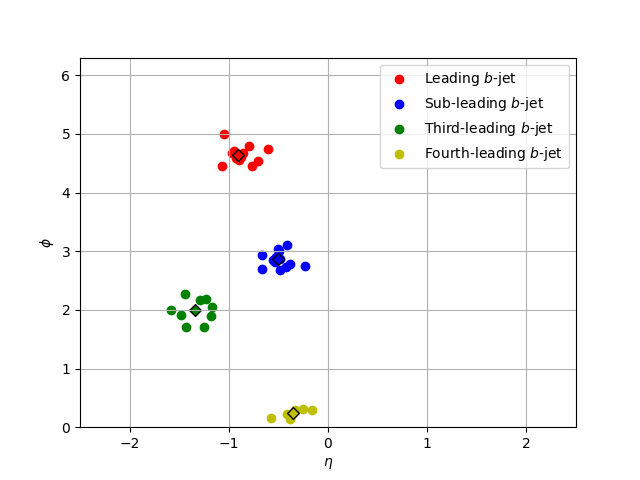
\includegraphics[scale=0.42]{plots/event_image_AK4.png}
	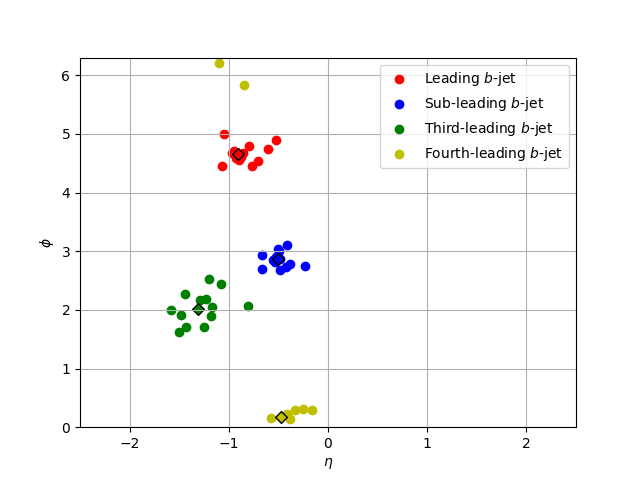
\includegraphics[scale=0.42]{plots/event_image_varR.png}
	 \end{center}
	\caption{The same MC event in $(\eta , \phi)$ space. Events have been clustered with (left) a fixed $R=0.4$, and (right) variable-$R$. The coloured points are the constituents of the corresponding $b$-tagged jet in the legend, and black outlined diamonds are at the overall $(\eta , \phi)$ coordinates of the overall $b$-jet.}
\label{fig:event_images}
\end{figure}

\begin{figure}[htb!]
	\begin{center}
	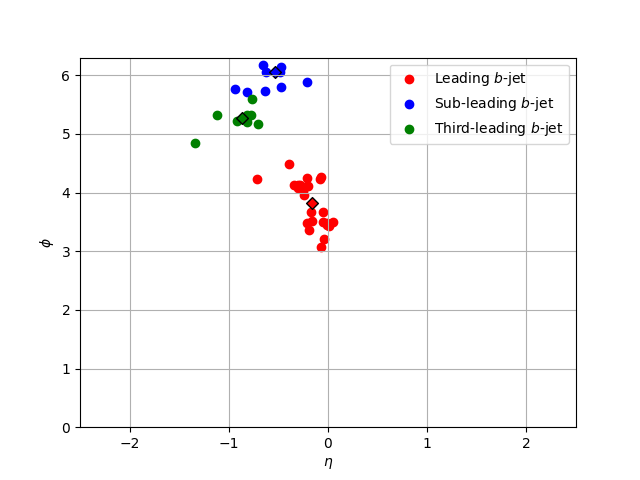
\includegraphics[scale=0.42]{plots/event_image_AK8_3bjets.png}
	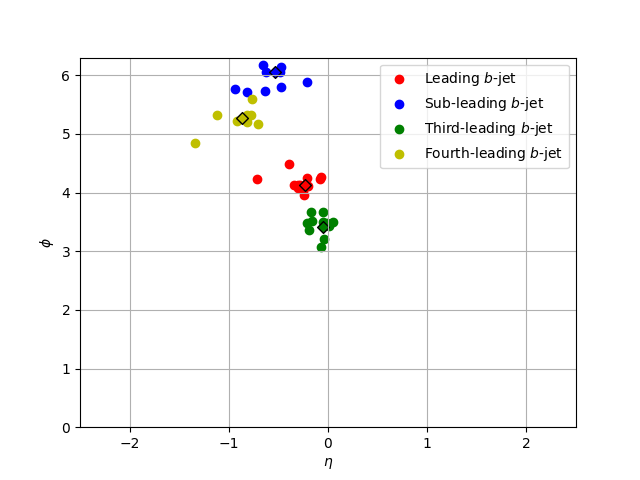
\includegraphics[scale=0.42]{plots/event_image_varR_4bjets.png}
	 \end{center}
	\caption{Same plot as in Fig.~\ref{fig:event_images}, however here the given event is clustered into three $b$-jets when a fixed $R=0.8$ is used (left), and four $b$-jets when we use a variable-$R$. The anti-$k_T$ algorithm is used in both cases.}
\label{fig:event_images2}
\end{figure}

\subsection{Implementation of $b$-Tagging}\label{btagging}
In this paper we implement a Monte Carlo (MC) informed $b$-tagger. For events clustered using a fixed-$R$ cone size, jets within angular distance $R$ from each parton level $b$-(anti)quark are searched for and tagged as appropriate. For scenarios where multiple jets are found, the closest is taken as the assignee for the $b$-tag. When the variable-$R$ approach is used, the size of the tagging cone is taken as the effective size of the jet $R_{\text{eff}}$ defined above.

In addition, when we consider the signal and background rates, we account for the finite efficiency of identifying a $b$-jet as well as the non-zero probability that $c$-jets and light-flavour plus gluon jets are mistagged as $b$-jets. We do so by firstly running jets through the MC $b$-tagger described above. However, in order to mimic finite efficiency effects, jets coming from $b$-(anti)quarks are then $b$-tagged with a $75\%$ success rate.
As for jets emerging from $c$-(anti)quarks, we assign to these a $10\%$ $b$-mistag rate. Finally, the remaining jets (lighter (anti)quark and gluon jetss), have a $1\%$ $b$-mistag rate applied.

The efficiencies described above are in line with the current rates at CMS, using the CMS $b$-tagger DeepCSV \cite{Sirunyan:2017ezt}, which quotes values of the $b$-tag efficiency rate, $c$-jet $b$-mistag rate, and light jet mistag rate of $68\%$, $12\%$ and $1.1\%$ respectively. Furthermore there is the CMS DeepJet tagger \cite{DEEPJET} which outperforms the DeepCSV tagger and shows $b$-tagging efficiencies higher than $68\%$ are reasonable.

We begin our analysis with a strict $p_T$ cut on $b$-jets of at least 30 GeV. Due to the rate at which signal is lost with these cuts we try a lighter $p_T$ cutflow informed by the $bb\mu^+\mu^-$ exotic Higgs analysis \cite{Sirunyan:2018mot}. Here, $p_T$ of the leading $b$-jet is required to have $>20$GeV, and others $p_T  >$15GeV. This reduced cutflow would require the implementation of a trigger with $p_T$ thresholds of 15, 10, 10, 10GeV for the four ($p_T$ ordered) $b$-jets. These $p_T$ thresholds are sufficiently below our jet $p_T$ requirement to enable $100\%$ efficiency in the trigger. 

\subsection{Simulation Details}
We consider two sample benchmark points, namely, $m_{h}$ = 40 GeV and 60 GeV, while  fixing $m_{H}$ = 125 GeV, within a 2HDM Type-II (2HDM-II henceforth), which have been tested against theoretical and experimental constraints by
using 2HDMC \cite{Eriksson:2010zzb}, HiggsBounds \cite{Bechtle:2013wla}, HiggsSignals \cite{Bechtle:2013xfa} as well as checking flavour contraints with SuperISO \cite{Mahmoudi:2009zz}. {We generate samples of ${\cal O}(10^5)$ events, with $\sqrt{s}=13 $ TeV.} The production and decay rates for the process $pp\to H\to hh\to b\bar b b\bar b$
are presented in Tab.~\ref{tab:params}, alongside the 2HDM-II input parameters. (Notice that the $H$ and $h$ decay widths are of order MeV, hence much smaller than the detector resolutions in two- and four-jet invariant masses, so that the Higgs states can essentially be treated as on-shell.) In the calculation of  the overall cross section, the  renormalisation and factorisation scales
were both set to be $H_{T}/2$, where $H_T$ is the sum of the transverse energy
of each parton. The Parton Distribution Function (PDF)  set  used was ${\tt NNPDF23_{\bf -}lo_{\bf -}as_{\bf -}0130_{\bf -}qed}$ \cite{Ball:2014uwa}.
Finally,
in order to carry out a realistic MC simulation, the toolbox described in Fig.~\ref{fig:toolbox} was used to generate and analyse events \cite{Alwall:2014hca,Sjostrand:2007gs,Conte:2012fm,Conte:2018vmg}\footnote{Note that we use the Leading Order (LO) normalisation for the signal cross sections here, for consistemcy with the fact that most of the  background ones  in our forthcoming analysis are only implemented at LO. While this affects our  final results on event rates and significances, we re-instate here that the main purpose of our paper is to assess the jet clustering performance, rather then the exact values of signal and backgrounds rates.}.

\begin{table}[!h]
\begin{center}
\hspace*{-1.35truecm}
\scalebox{0.8}{
\begin{tabular}{ |c|c|c|c|c|c|c|c|c|c| }
 \hline
 $m_h$ (GeV) & $m_A$ (GeV) & $m_{H^{\pm}}$ (GeV) & BR($H\rightarrow hh$) & BR($h\rightarrow b\overline{b}$)&$\sigma$(pb)  \\
 \hline
40 & 600 & 600 &  3.231 $\times 10^{-2}$ &9.066$\times 10^{-1}$&3.542$\times 10^{-1}$\\
 \hline
60 & 620 & 400 & 6.764 $\times 10^{-1}$ &8.610 $\times 10^{-1}$&6.688\\
\hline
\end{tabular}
}
\caption{\label{tab:params} The 2HDM-II  parameters and cross sections of the process  in Fig. \ref{fig:diagram} used here. Note that in both cases we fix $\lambda_6 = \lambda_7 = 0$, $m_{12}^2 = 4000$, $\tan\beta = 1.6$, $\sin (\beta - \alpha )$, and $m_H = 125$GeV (in line with the SM Higgs).}
\end{center}
\end{table}

\vspace*{1em}
\tikzstyle{node} = [rectangle, rounded corners, minimum width=3cm, minimum height=1cm,text centered, draw=black]
\tikzstyle{arrow} = [thick,->,>=stealth]

%\hspace*{-4em}
\begin{figure}[htb!]
\centering
\hspace*{-0.5truecm}
\begin{tikzpicture}[node distance=1.5cm]
\node (step1) [node] {Generate signal events of $gg \rightarrow H \rightarrow h h \rightarrow b b \bar{b} \bar{b}$ using {\tt MadGraph5@NLO v2.6.3.2}};
\node (step2) [node, below of=step1] {Shower and hadronise parton level events using {\tt Pythia8 v8.243}};
\node (step3) [node, below of=step2] {Perform jet reconstruction, apply cuts and carry out analysis using {\tt MadAnalysis5 v1.8.5}};

\draw [arrow] (step1) -- (step2);
\draw [arrow] (step2) -- (step3);
\end{tikzpicture}
\caption{Description of the procedure used to generate and analyse MC events. }
\label{fig:toolbox}
\end{figure}

%\newpage
%\section{Cutflow}
Before introducing the sequences of cuts that we have adopted here,
some discussions are in order on their possible choice. In existing
four $b$-jet analyses by the ATLAS and CMS collaborations, seeking to
extract chain decays of Higgs bosons like the ones considered here
from of the background, rather restrictive cuts have been used for the
ensuing fully hadronic signature. Taking CMS as an example, upon
enforcing the same $p_T$ cuts on $b$-jets as in
Ref.~\cite{Sirunyan:2019jud}, which are as shown in
Fig.~\ref{fig:cutflow}, we noticed that the signal selection
efficiency was too low (in various respects, as described later) to
enable one to create a MC sample suitable for experimental analysis
assuming Run 2 and 3 luminosities. We explored the possibility of using
lower $p_T$ cuts on the jets and finally used $p_T$ cuts used by the
CMS experiment in  in the analysis of $b\bar
b\mu^+\mu^-$ final states (also emerging from Higgs cascade decays) of
Ref.~\cite{Sirunyan:2018mot}. We replaced the
starred $(*)$ cut $p_T>30$ GeV on each reconstructed $b$-jet in
Fig.~\ref{fig:cutflow} as described in Section.~\ref{btagging} with 
a cut of $p_T$ $>$ 20 GeV for the leading $b$-jet with all others 
required to have $p_T >$ 15 GeV. We will discuss the pros and cons of each of the
cutflows in the forthcoming section.

\vspace*{1em}
\tikzstyle{node} = [rectangle, rounded corners, minimum width=3cm, minimum height=1cm,text centered, draw=black]
\tikzstyle{arrow} = [thick,->,>=stealth]

%\hspace*{-4em}
\begin{figure}[!t]
\centering
\hspace*{-1.05truecm}
\begin{tikzpicture}[node distance=1.5cm]
\node (cut1) [node] {Remove all final state particles with a $p_T < 0.5$ GeV and $|\eta| > 2.5$};
\node (cut2) [node, below of=cut1] {Perform jet reconstruction and $b$-tagging in {\tt fastjet} \cite{Cacciari:2011ma}, with specified clustering algorithm and $\Delta R$};
\node (cut3) [node, below of=cut2] {Remove $b$-jets with $p_T < 30$ GeV $(*)$};
\node (cut4) [node, below of=cut3] {Remove $b$-jets whose energy content due to electrons(muons) is greater than  90(80)\%, respectively.};
\node (cut5) [node, below of=cut4] {Remove $b$-jets whose energy content due to neutral hadrons and photons is greater than 90\%.};
\node (cut6) [node, below of=cut5] {Remove $b$-jets with zero charged hadron energy};
\node (cut7) [node, below of=cut6] {Remove $b$-jets with only one constituent};

\draw [arrow] (cut1) -- (cut2);
\draw [arrow] (cut2) -- (cut3);
\draw [arrow] (cut3) -- (cut4);
\draw [arrow] (cut4) -- (cut5);
\draw [arrow] (cut5) -- (cut6);
\draw [arrow] (cut6) -- (cut7);
\end{tikzpicture}
\caption{Description of our initial procedure for jet clustering, $b$-tagging and selection of jets. Notice that the starred cut $(*)$ will eventually be modified in our optimised $b$-jet selection. Also note that our analysis is performed at particle level rather than detector, so truth level MC information is used for cuts on jet constituents.}
\label{fig:cutflow}
\end{figure}
%%%=====================================================================================================
%\newpage
%\section{Jet Reconstruction and b-tagging}
\section{Results}
%%%================================================
In this section we present the results for our signal at both the parton and detector level. In the latter case, we also discuss the dominant backgrounds, due to QCD $4b$ production, $gg,q\bar q\to Zb\bar b$ and $gg,q\bar q\to t\bar t$\footnote{In fact, we have checked that the additional noise due to
$t\bar t b\bar b$ events as well as hadronic final states emerging from $W^+W^-, W^\pm Z$ and $ZZ$ production and decay are negligible, once mass reconstruction around $m_h$ and $m_H$ are enforced.}.

\subsection{Parton Level Analysis}

At the Matrix Element (ME) level, all the events have four $b$-quarks originating
from the decay of the two light Higgs boson ($h$). The mass difference between
the heavy and light Higgs states leads to boosted $b$-quarks,
therefore, we plot the $R$ separation between the $b$-quarks coming from
the same light Higgs state (see upper panel of Fig.~\ref{fig:parton_higgs}).  The two distributions corresponding to $m_h=40$ and 60 GeV are markedly different. This can be understood as follows.
%%%%%%%%%%%%%
%Light Higgs bosons are relatively boosted because of the mass difference wrt to the heavy Higgs boson,
%and thus the b-quarks are more boosted (see the lower panel (left plot) of
%figure \ref{fig:parton}).
%%%%%%%%%%%%%
In general, the angular separation between the decay products $a$ and $b$  in the resonant process
 $X \to a b$ can be approximated as $\Delta R (a,b) \sim \frac{2 m_{X}}{p^{X}_T}$. Hence, we plot in the lower left panel of
Fig.~\ref{fig:parton_higgs} the transverse momentum of each of the $h$ bosons.
For $m_h$ = 60~GeV, the light Higgs boson has less $p_T$ than for lower values (owing to the smaller $m_H-m_h$ mass difference), therefore, the $b$-quarks
are more widely separated in this case, compared to $m_h=40$. In the light of this, we can
already conclude that there is a strong correlation between the lightest Higgs boson mass and
the cone size of the jet clustering algorithm that ought to be used. In particular, we can say  that, in order to maximise the number of jets\footnote{This is done in view of background rejection.} for different choices of the light Higgs boson
mass, we need to vary the jet radius parameter. That is, a fixed jet radius parameter may not
be suitable here for all $m_h$ choices. In the lower right panel of Fig.~\ref{fig:parton_higgs}, we finally plot the
$\Delta R$ separation between the two light Higgs states. For a light Higgs boson mass of $m_h = 40$ GeV, it is clear (since $\Delta R\approx \pi$) that
the $H \to h h $ decay is dominantly back-to-back (in the laboratory frame). However, for $m_h = 60$ GeV,  there is a double peak structure. This occurs due to a recoil effect from initial state radiation (ISR), which only becomes apparent at the mass boundary where $m_H \simeq 2m_h$. The inability of the two emerging $h$ states to fly apart implies some overlapping of
the $b$-quark momenta. Hence, we expect that the signal, upon enforcing  a jet clustering algorithm, will have a rather high $b$-jet multiplicity, so long that the two $b$-jets stemming from $h$ decays are resolved, unless detector acceptance and signal selection cuts reduce it, which is quite possible given the light masses considered for  the $h$ state in relations to typical jet $p_T$ thresholds used in applying $b$-tagging.  We will investigate this next.

As a final study, in fact, the $p_T$ of the $b$-quarks is plotted. This is done in Fig.~\ref{fig:parton_b}.
From the top histogram we can see that in both mass configurations the $b$-quarks have a wide range of $p_T$'s and hence one would expect the resulting jets to have a similar spread of $p_T$'s. In particular, we also plot the highest and lowest $p_T$'s amongst the $b$-quarks in a given event (bottom-left and bottom-right frames, respectively). Further to the discussion in section~\ref{JetClusteringwithVariableR}, one would therefore expect the resulting spread of radiation from each signal $b$-quark to vary in  solid angle and hence the resulting jets be of differing sizes. This thus motivates the need for a jet reconstruction sequence that behaves sensibly for jets of various cone sizes. Therefore, in the next section, we firstly test how jet clustering with fixed-$R$ input behaves and then introduce the variable-$R$ algorithm.



\begin{figure}[htb!]
	\begin{center}
	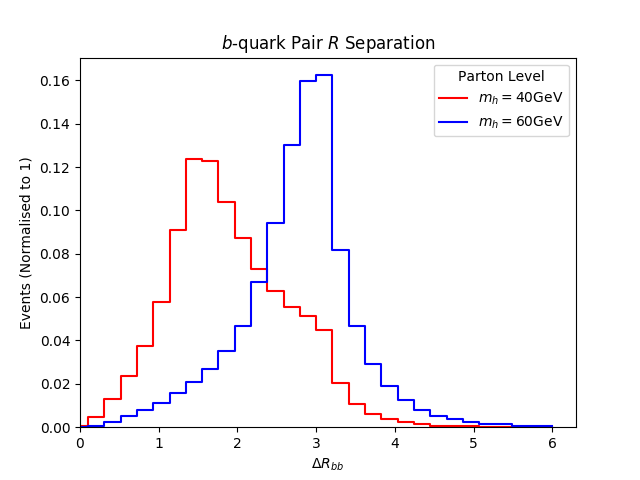
\includegraphics[scale=0.42]{plots/parton/delRbb.png}\\
%          \hspace*{-0.4cm}
	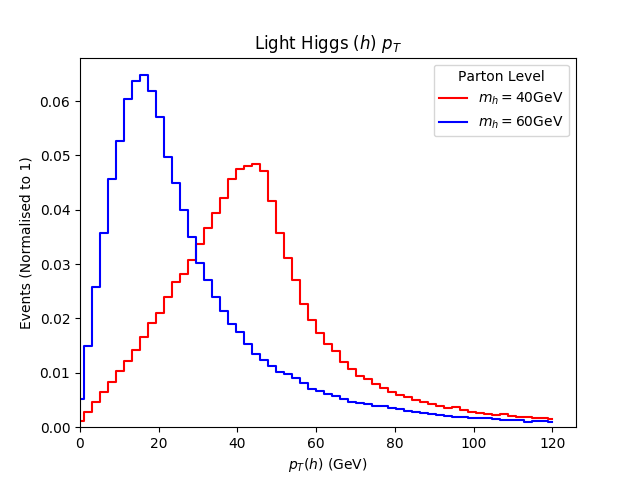
\includegraphics[scale=0.42]{plots/parton/LHiggs_pt.png}
	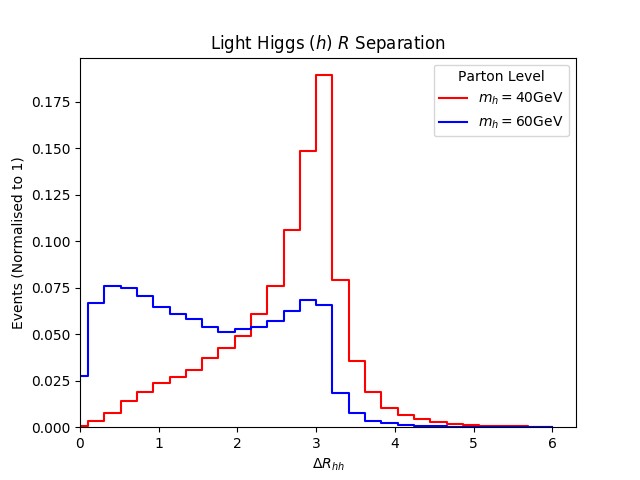
\includegraphics[scale=0.42]{plots/parton/LHiggs_DelR.png}
	 \end{center}
	\caption{Upper panel: the $\Delta R$ distribution between the
two $b$-partons originating from the same $h$. Lower panels: (Left)
the $p_T$ distribution of the light Higgs boson $h$ originating from $H$ decay;
(Right) the $\Delta R$ distribution between the two $h$ states originating from the
$H$ decay. The following two mass choices have been considered: $m_h=40$ and 60 GeV. No (parton level) cuts have been enforced here. }
\label{fig:parton_higgs}
\end{figure}

\begin{figure}[htb!]
	\begin{center}
	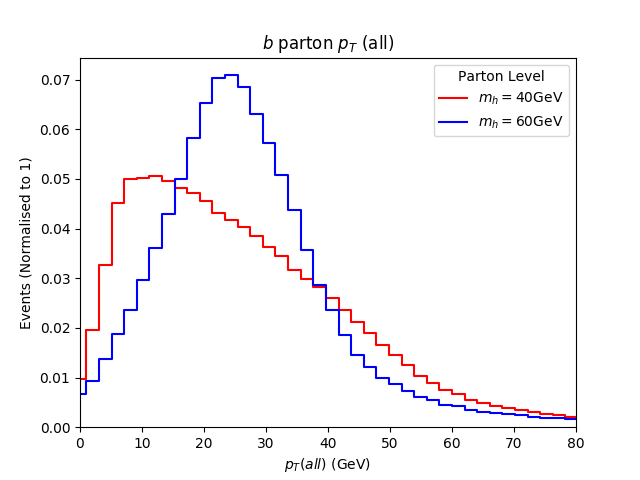
\includegraphics[scale=0.42]{plots/parton/b_pt.png}\\
%          \hspace*{-0.4cm}
	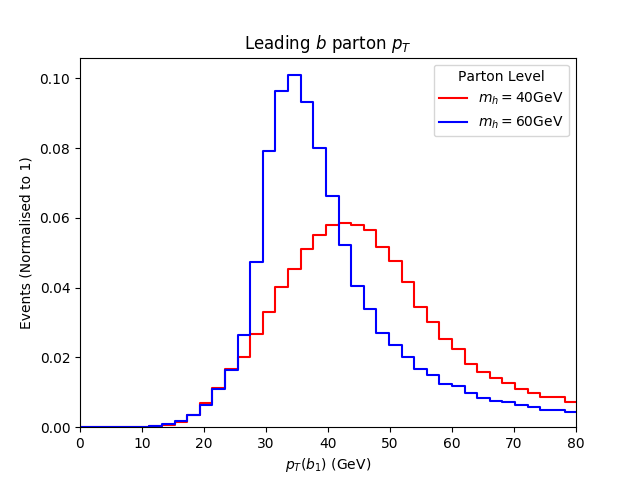
\includegraphics[scale=0.42]{plots/parton/b1_pt.png}
	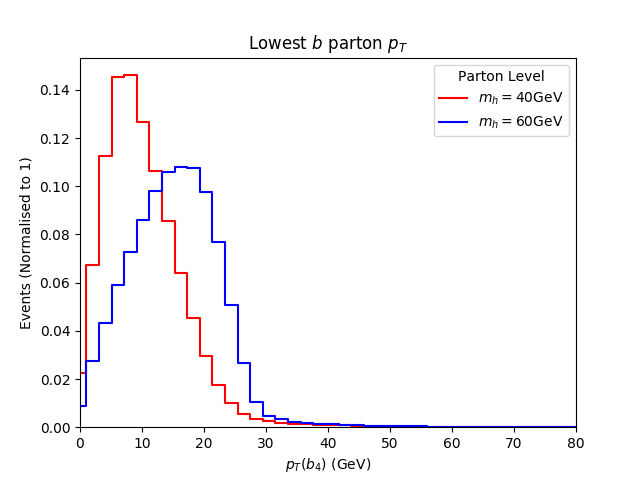
\includegraphics[scale=0.42]{plots/parton/b4_pt.png}
	 \end{center}
	\caption{Upper panel: the $p_T$ distribution for all $b$-quarks. Lower panels: (Left) highest $p_T$ amongst the $b$-quarks; (Right) lowest $p_T$
amongst the $b$-quarks. No (parton level) cuts have been enforced here.}
\label{fig:parton_b}
\end{figure}

%%%%%%%%%%%
%\end{document}
%%%%%%%%%%%

%%%================================================================
\subsection{Hadron Level Analysis}
We start this section by investigating  the performance of jet reconstruction and $b$-tagging, in particular, in order
to see how often the entire signal of four $b$-jets is selected. Initially,  a
baseline analysis without cuts is performed, using the anti-$k_T$ jet algorithm \cite{Cacciari:2008gp} with  (fixed) jet
radius parameters $R = 0.4$ and 0.8. (The results for the CA scheme are very similar, so we refrain from presenting them here.)
The  corresponding multiplicity of $b$-tagged jets  is plotted in the top
left frame of Fig.~\ref{fig:nbjets}, where no $p_T$ cut has been imposed on the $ b$-jets or to its constituents prior to clustering, thereby exemplifying a 'perfect' detector.
We find that the majority of the events include four $b$-tagged jets. However, notice that,
if we follow typical jet selection cuts used in experimental analyses of $4b$ final states (see our Fig.~\ref{fig:cutflow}),
even with our MC based $b$-tagger in action, it is not always
possible to reconstruct all the four expected $b$-jets (see top-right frame of
Fig.~\ref{fig:nbjets}), as we notice a significant shift towards smaller $b$-jet multiplicities in this case, the more so the lighter the $h$ mass. The pattern is rather similar for $R=0.4$ (bottom frames of Fig.~\ref{fig:nbjets}), albeit less so the heavier the $h$ mass. Altogether the shift is substantial in both $R$ cases, to the extent that, in  a scenario where the LHC deploys a
search with the cuts listed in  Fig.~\ref{fig:cutflow}, the majority of signal events is lost and this is specifically due to the severe $p_T$ cuts,
as can be seen from the (cumulative) $p_T$ distribution of all $b$-jets before cuts,  Fig.~\ref{fig:bjetpt}. In fact, from here, it is clear that, no matter the final $b$-jet multiplicity, a $p_T>30$ GeV cut on all reconstructed jets  is very damaging, thereby hinting that somewhat looser cuts on the hadronic system may be desirable (as mentioned in the previous section)\footnote{In fact, we should further notice that the left frames of
Fig.~\ref{fig:nbjets}, i.e., in absence of any cuts, also serve the purpose of quantifying the efficiency of our $b$-tagging performance.}.  Results for the CA jet algorithm (whatever the $R$ value) are not significantly different for any of the observables discussed.
%
%
\begin{figure}[t!]
%	\centering
	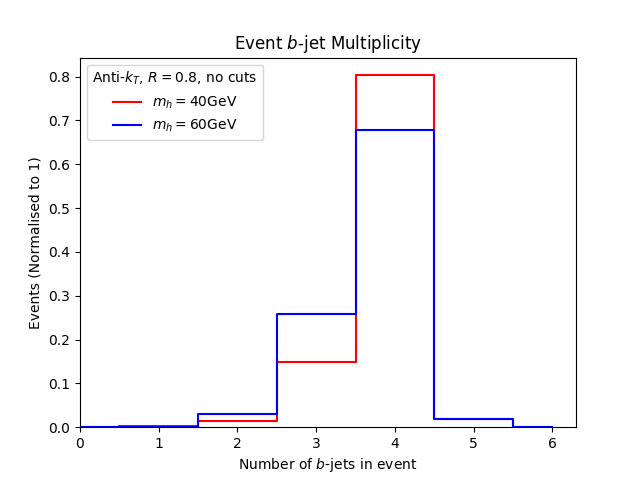
\includegraphics[scale=0.5]{plots/nbjets_AK8_nocuts.png}
	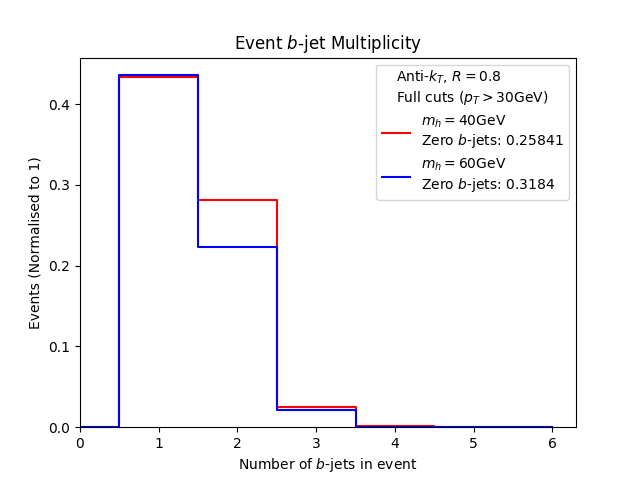
\includegraphics[scale=0.5]{plots/nbjets_AK8_pt30.png}
	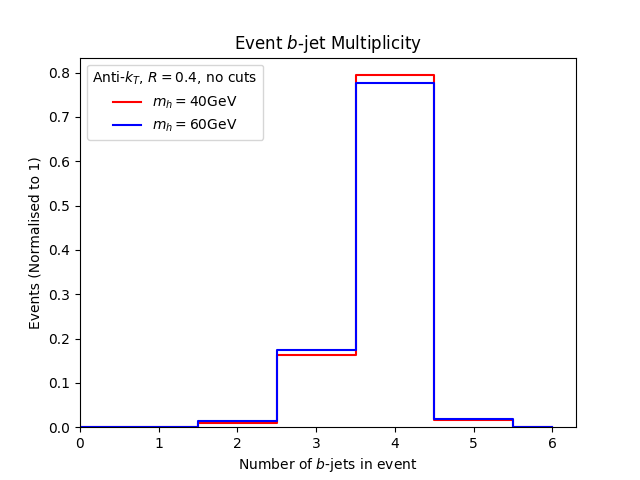
\includegraphics[scale=0.5]{plots/nbjets_AK4_nocuts.png}
	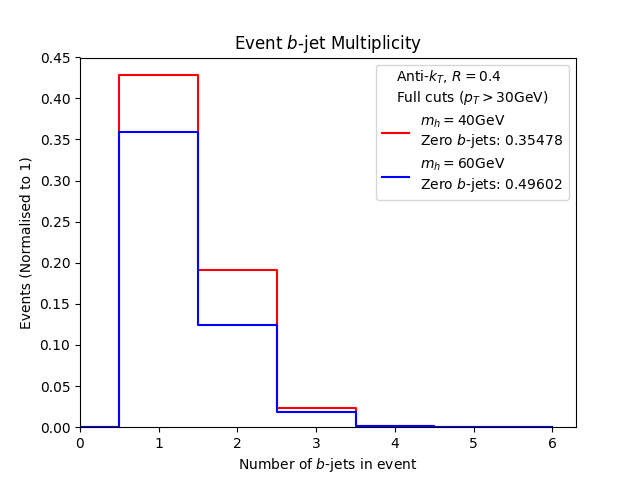
\includegraphics[scale=0.5]{plots/nbjets_AK4_pt30.png}
	\caption{The distributions of $b$-jet multiplicities when no cuts are imposed on the jets (left panels) and with the full cutflow described  in
Fig~\ref{fig:cutflow} (right panels). Top(Bottom) panels are for $R = 0.8(0.4)$. Here, we have used the anti-$k_T$ jet clustering algorithm. Note that events containing zero $b$-jets are not plotted but included in the legend, in the case of no cuts being applied all events contain at least one $b$-jet.}
\label{fig:nbjets}
\end{figure}
%
\begin{figure}[htb!]
	\centering
	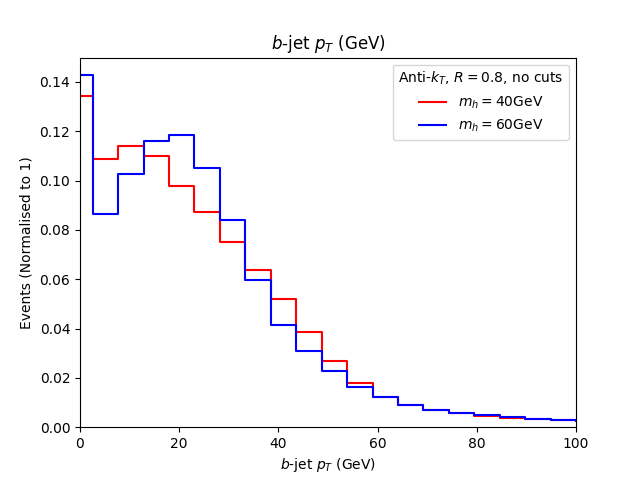
\includegraphics[scale=0.6]{plots/bjetpt_AK8_nocuts.png}
	\caption{Transverse momentum distribution of all $b$-jets with no cuts imposed on the jets or on the final state hadrons. We have used here $R=0.8$, though the pattern is similar for $R=0.4$. Here, we have used the anti-$k_T$ jet clustering algorithm.}
\label{fig:bjetpt}
\end{figure}

Before addressing the issue of an alternative selection of the hadronic system,  we want to discuss some kinematic features of the surviving events.
%%%%%%%%%%%%%%%%%%%%%%%%%
%Specifically, when we reconstruct the invariant masses  of two- and four-jet systems (see Fig.~\ref{fig:invmass1}) in the attempt to extract both the light %and heavy Higgs resonances starting from the subset of events with four $b$-tagged jets {\textcolor{red}{SM: please confirm that this is the case}} %{\textcolor{blue}{BF: We do not attempt to extract any masses from the full cut samples, as this requires at least three b jets to be present, with full cuts %the statistics are not good enough to do this. I suggest a replacement for this paragraph below}}, these are indeed present  in the relevant mass %distributions. However, while the two-jet mass distributions develop a shift of the peaks (from both $m_h=40$ and 60 GeV)
% by a few GeV, the same effect on the four-jet ones is more substantial, amounting to tens of GeV shifts from $m_H=125$ GeV. The effect is more marked %for smaller (lower frames in    Fig.~\ref{fig:invmass1}) than larger (upper frames in  Fig.~\ref{fig:invmass1}) cone sizes. Hence, we further conclude that %the standard $4b$ cuts of Fig.~\ref{fig:cutflow} also have the  effect of distorting the Higgs mass peaks, though this may also be due to the choice made %of a jet clustering algorithm with fixed cone size, as hinted by Fig.~\ref{fig:parton} (we will come back to this aspect later).
%%%%%%%%%%%%%%%%%%%%%%%%%
Specifically, the selection that we implement to construct two- and four-jet mass distributions (described below) requires that we select at least three $b$-jets. The poor statistics due to these strict cuts does not allow for this, as  visible in Fig.~\ref{fig:nbjets}. Thus, as a  test of our ability to reconstruct $m_h$ and $m_H$ from two- and four-jet systems, we present distributions for samples before cuts are applied, see Fig.~\ref{fig:invmass1}. In order to seek out a $m_h$ resonance in the mass of $b$-jet pairs, we select events with three or four $b$-jets. For those with three, we compute $m_{bb}$ for all possible pairs and select the pair minimising $|m_{bb}-m_h|$. In the case where all four $b$-jets are reconstructed, the same selection is made, but the left-over $b\bar b$ pair is also included so as to account for the presence of the second light Higgs state. (Herein, tails are due to inefficiency in this pairing technique and also to fixed cone effects in jets for which $\Delta R$  is smaller than $R$.)
%
Notice the two-jet mass distributions develop a shift of the peaks (from both $m_h=40$ and 60 GeV), by a few GeV, and that the same effect is present on the four-jet ones (and is even more substantial), amounting to tens of GeV shifts from $m_H=125$ GeV. The effect is more marked for smaller (lower frames in    Fig.~\ref{fig:invmass1}) than larger (upper frames in  Fig.~\ref{fig:invmass1}) cone sizes. We are thus motivated to consider an alternative to a reconstruction using a fixed cone size. Again, results for the CA jet algorithm are not significantly different for any of the observables presented here using the anti-$k_T$ algorithm.
%
%
\begin{figure}[t!]
%	\centering
	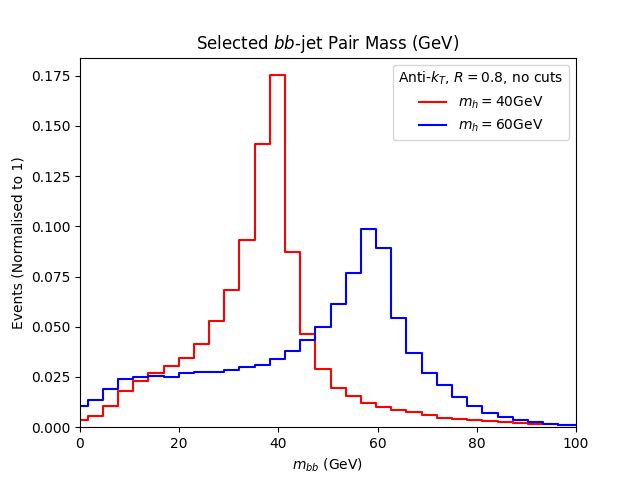
\includegraphics[scale=0.5]{plots/bbmass_AK8_nocuts.png}
	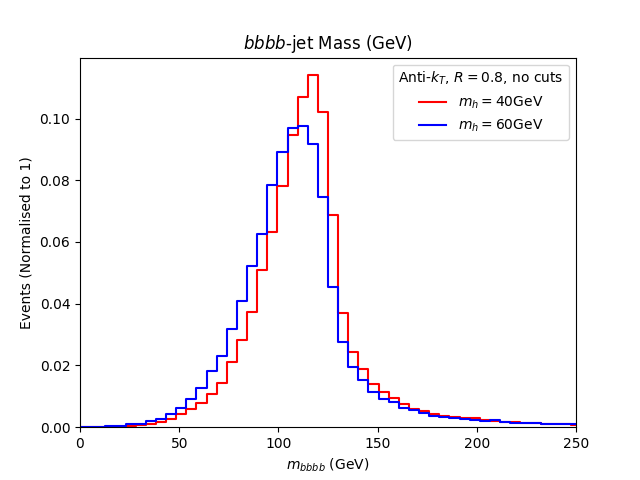
\includegraphics[scale=0.5]{plots/bbbbmass_AK8_nocuts.png}
	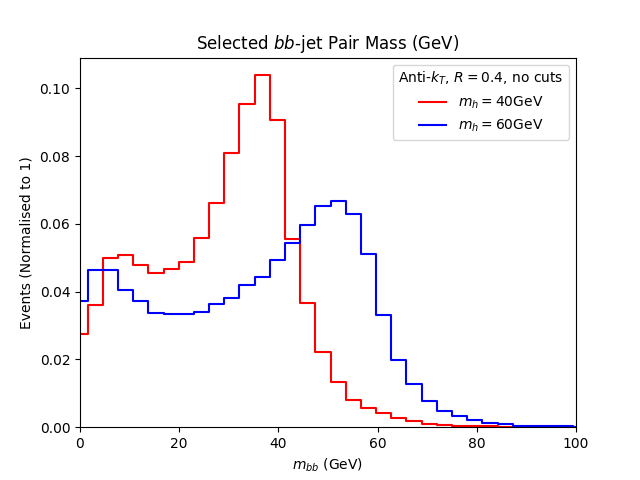
\includegraphics[scale=0.5]{plots/bbmass_AK4_nocuts.png}
	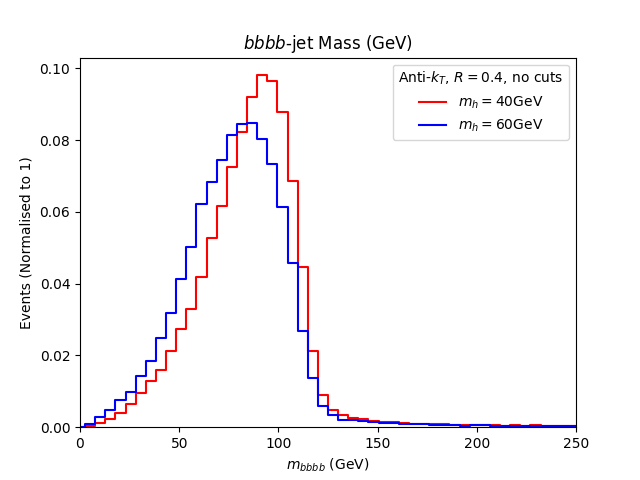
\includegraphics[scale=0.5]{plots/bbbbmass_AK4_nocuts.png}
	\caption{The distributions in invariant mass of two (left panels) and four (right panels) $b$-tagged jets. No cuts have been implemented here.
Top(Bottom) panels are for $R = 0.8(0.4)$. Here, we have used the anti-$k_T$ jet clustering algorithm.}
\label{fig:invmass1}
\end{figure}
%
%\newpage
%To simulate a more realistic analysis the cutflow defined above is applied
%\begin{figure}[h!]
%	\centering
%	\includegraphics[scale=0.9]{plots/nbjets_pt30.png}
%	\caption{$b$-jet multiplicity with full cutflow defined above.}
%\label{fig:diagram}
%\end{figure}


%\newpage

{{With an improvement of the $b$-jet multiplicity in mind, we adopt the lesser cuts described at the end of the previous section:}} i.e., the
leading $b$-jet has $p_T$ $>$ 20 GeV while the remaining ones are required to  have $p_T >$ 15 GeV \cite{Sirunyan:2018mot}. With this
revised selection cuts (henceforth, `reduced cuts'), the $b$-jet multiplicity distribution changes significantly, see Fig.~\ref{fig:nbjet_ptcut}. That is, we notice distributions which consistently (i.e., for both $R$ values adopted) display a better efficiency  of the new $p_T$ cuts  in selecting a higher number of $b$-jets
 (compare to the right frames in Fig.~\ref{fig:nbjets}).  In particular, the presence of more events containing all four $b$-jets from the signal
allows one also to better reconstruct the Higgs masses in multi-jet mass distributions, see Fig.~\ref{fig:invmass2}.



\begin{figure}[t!]
%	\centering
	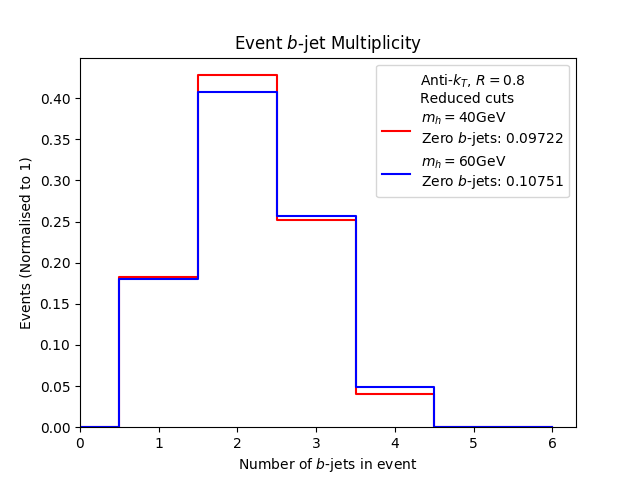
\includegraphics[scale=0.45]{plots/nbjets_AK8_lowptcut.png}
	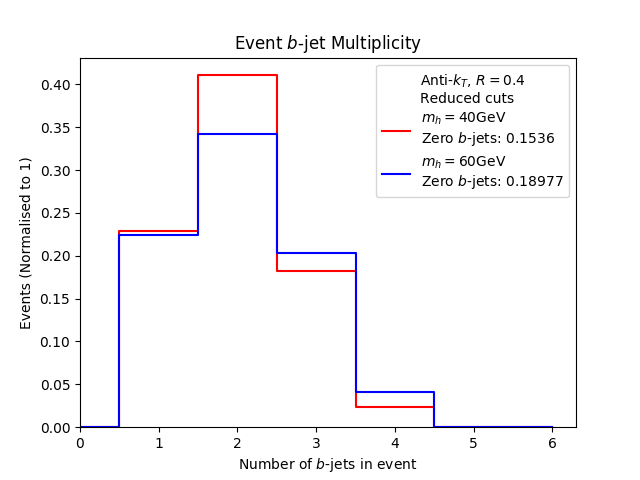
\includegraphics[scale=0.45]{plots/nbjets_AK4_lowptcut.png}\\
%	\includegraphics[scale=0.45]{plots/nbjets_CA8_lowptcut.png}
%	\includegraphics[scale=0.45]{plots/nbjets_CA4_lowptcut.png}
	\caption{The distributions of $b$-jet multiplicities when the cuts in $p_T$ discussed at the end of the previous section have been implemented here.
Left(Right) panel is for $R = 0.8(0.4)$.
The anti-$k_T$ jet clustering algorithm has been used throughout. Note that events containing zero $b$-jets are not plotted but included in the legend.}
\label{fig:nbjet_ptcut}
\end{figure}

%\newpage

%
\begin{figure}[htb!]
	%\centering
	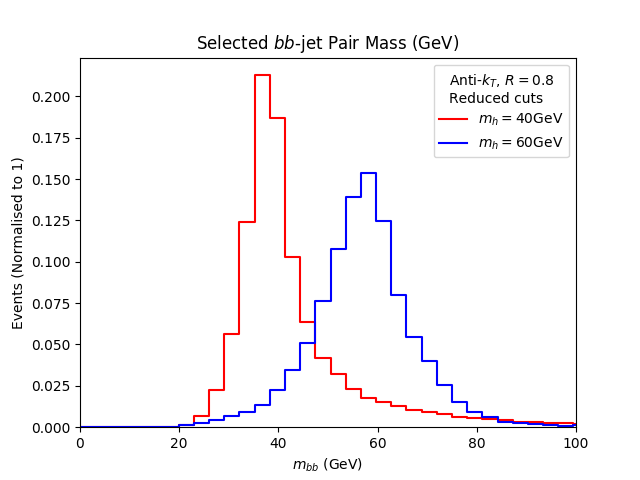
\includegraphics[scale=0.5]{plots/bbmass_AK8_lowptcut.png}
	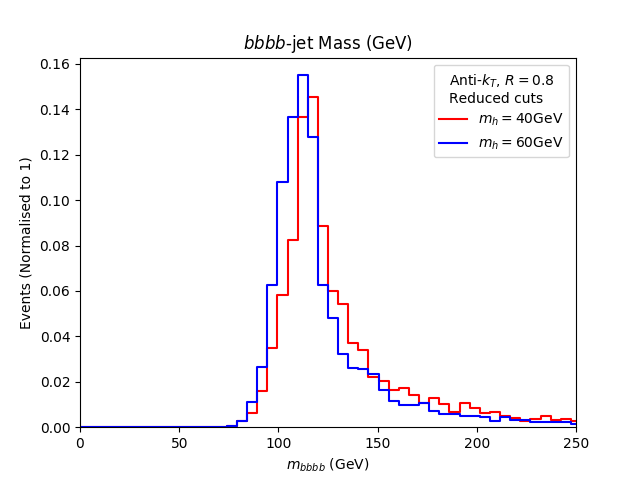
\includegraphics[scale=0.5]{plots/bbbbmass_AK8_lowptcut.png}
	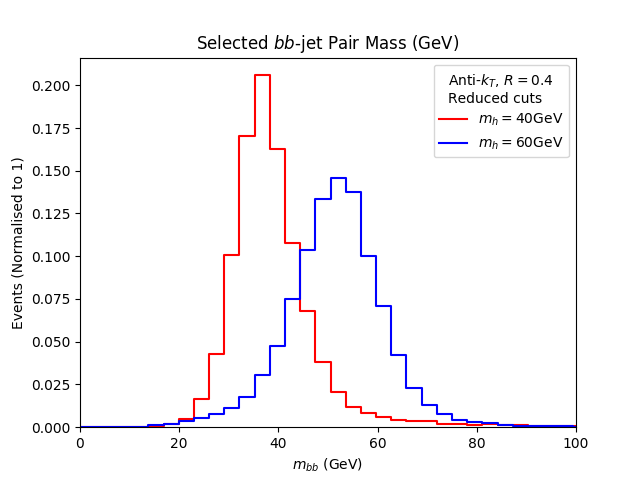
\includegraphics[scale=0.5]{plots/bbmass_AK4_lowptcut.png}
	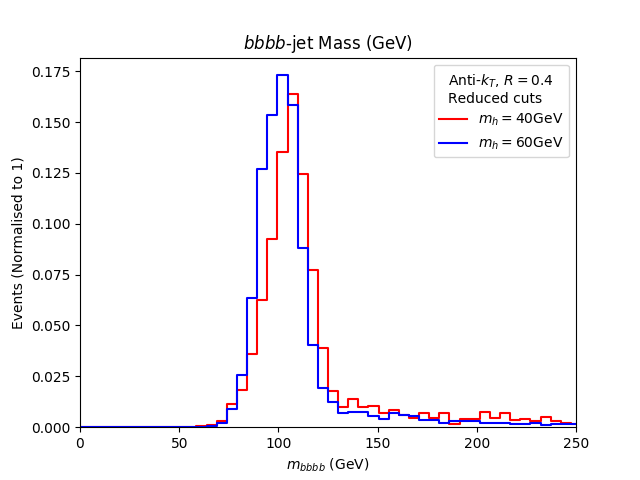
\includegraphics[scale=0.5]{plots/bbbbmass_AK4_lowptcut.png}
	\caption{The distributions in invariant mass of two (left panels) and four (right panels) $b$-tagged jets, in presence of the
  reduced $p_T$ cuts on the $b$-jets.
Top(Bottom) panels are for $R = 0.8(0.4)$. Here, we have used the anti-$k_T$ jet clustering algorithm.}
\label{fig:invmass2}
\end{figure}
%

%================================
%1. fix R = 0.8, explain $b$-jet multiplicity with/without pt cuts, mass reco, not so good. ptcut is not good.
%2. revised cuts folowing cms paper, 4 $b$-jet samples improve, reco imporved merginally ...
%4. variable-$R$, how does it work, effective values, mass reco, nice peaks ...


%%------------------------------------------------------------------------------------------
%%%---- variable-$R$ approach
%%------------------------------------------------------------------------------------------


Before moving on to a signal-to-background analysis in presence of reduced $p_T$ cuts on the $b$-jets,
however, there is a further way of improving the
proportion of events containing larger $b$-jet multiplicities. Referring back to Fig.~\ref{fig:nbjets},
where, even without cuts, a significant number of $b$-jets is already lost in the process
of jet reconstruction and tagging, and further noticing, from Fig.~\ref{fig:parton_higgs}, that  the cone size plays a crucial role in this respect,
it is not surprising that  using a `{variable-$R$}' approach to jet clustering (and hence tagging), like the one of Ref.~\cite{Krohn:2009zg},
recovers a better multiplicity behaviour from
the $b$-jet sample before cuts are applied. In this approach, the clustering process is modified, as explained in a previous section, so that one
%%%%%%%%%%%%%%%%%%%
%rather than defining a fixed jet radius $R$, this parameter is replaced with an effective jet radius
%$R_{\text{eff}} =  {\rm min} (\frac{\rho}{p_T}, R_{\rm max})$, where $\rho$ is a dimensionfull parameter
%and $R_{\rm max}$ is the cut-off for the jet radius. The later is used for
%%%%%%%%%%%%%%%%%%%
can more efficiently avoid events with very wide jets at low $p_T$. The parameter $\rho$ can be
optimised to obtain maximum desired sensitivity. Furthermore, other parameters such as $R_\text{min/max}$, which are cut offs for the minimum and maximum allowed $R_\text{eff}$ (that is, if a jet has $R_\text{eff} > R_\text{max}$, it is overwritten and set to $R_\text{eff} = R_\text{max}$, and equivalent for $R_\text{min}$). In order to select the optimal choice of $\rho$, a scan over various values is performed, the  results of which are in Fig.~\ref{fig:rhoscan}. To measure each $\rho$ choice, events are reconstructed and tagged using the standard procedure, with the reduced cutflow described in Fig.~\ref{fig:cutflow}. The $b$-jets are then put into pairs based on those best reconstructing the relevant Higgs mass and events are then put through the selection process described later in Fig.~\ref{fig:selection}, after which the number of events passing the selection (normalised to one) is plotted.

\begin{figure}[htb!]
	%\centering
	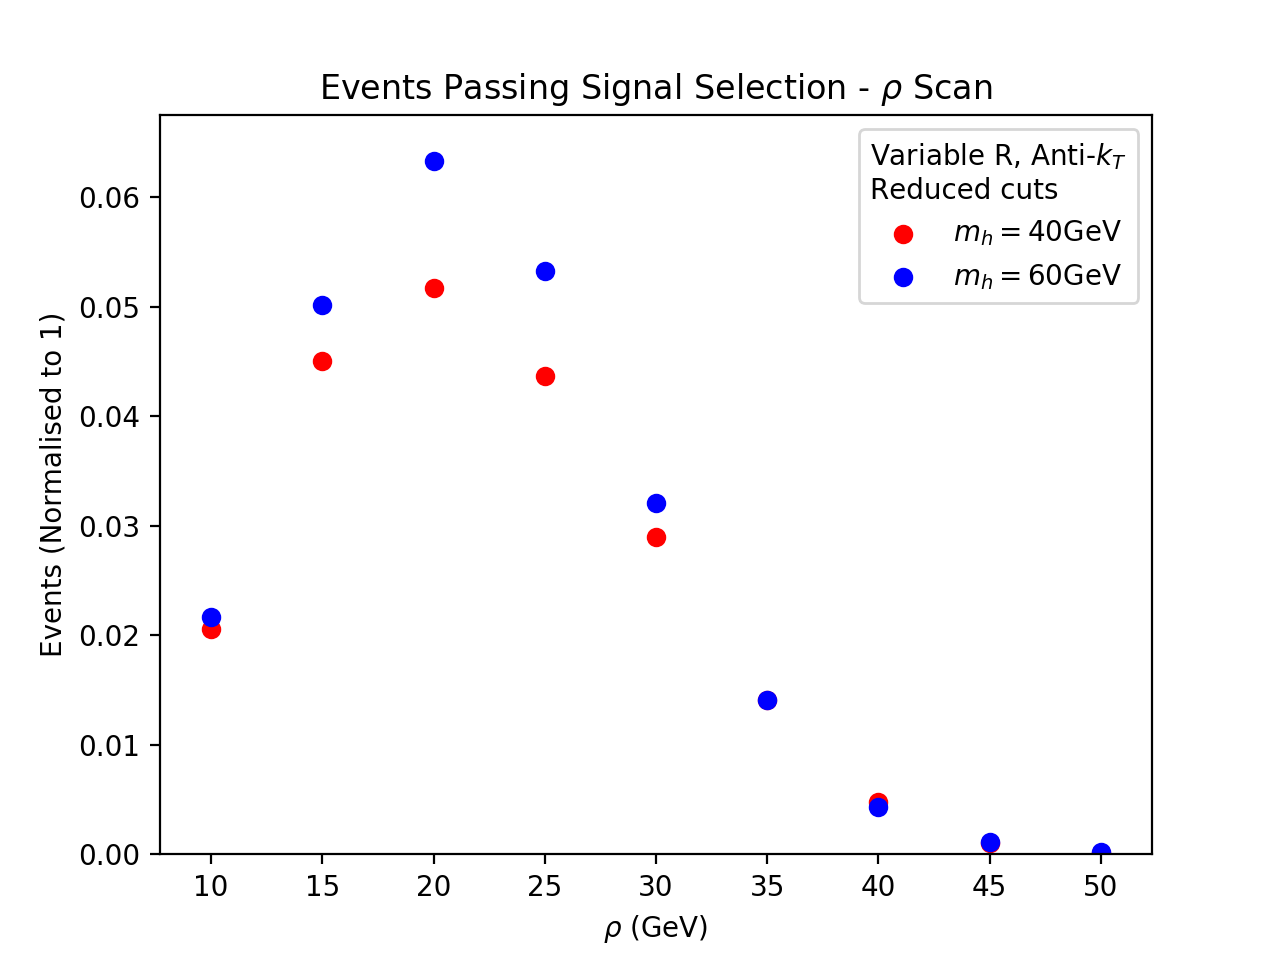
\includegraphics[scale=0.45]{plots/rho_scan_results_1050.png}
	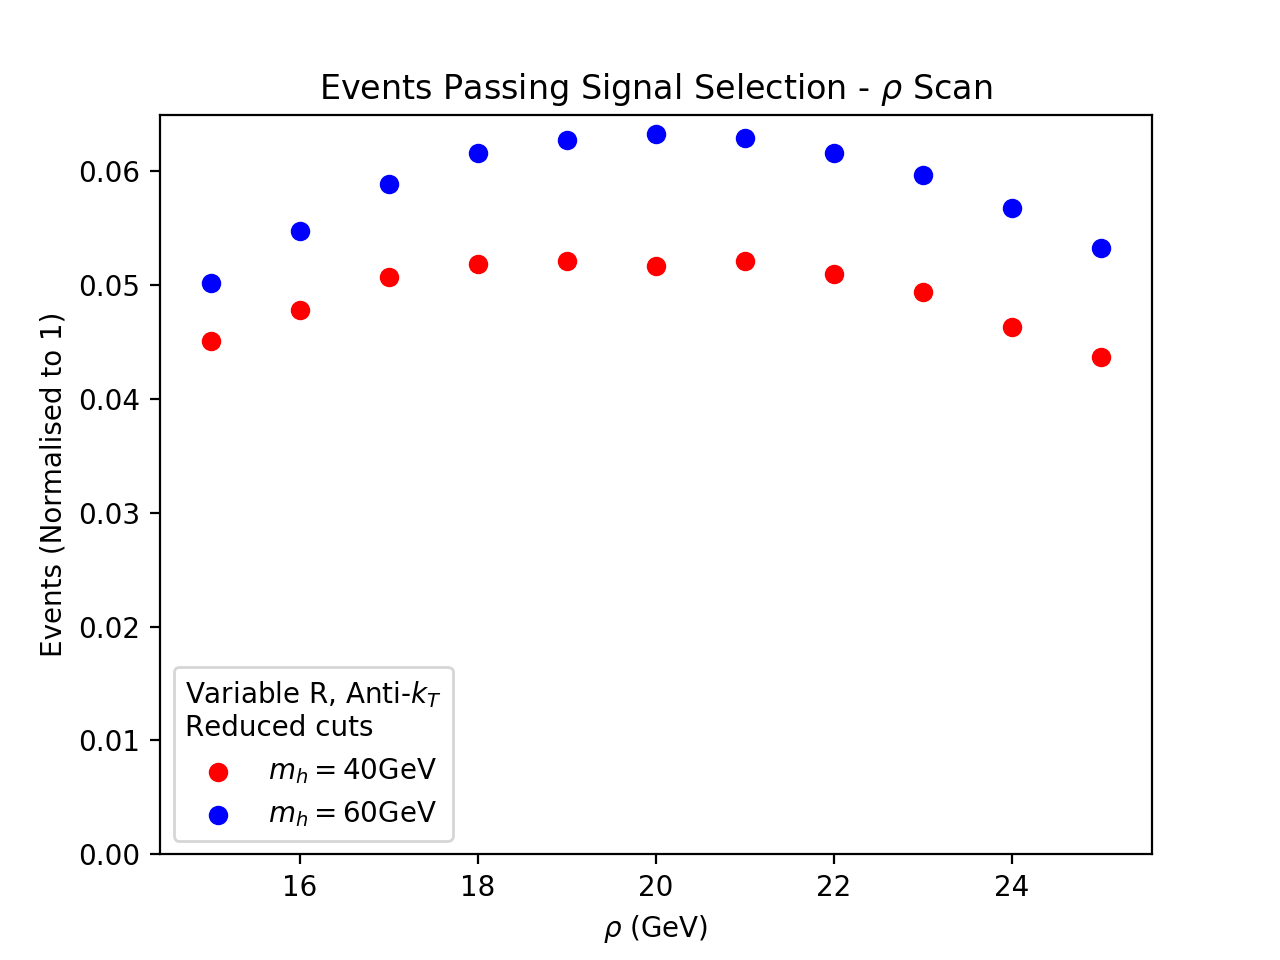
\includegraphics[scale=0.45]{plots/rho_scan_results_1525.png}
	\caption{Scan over the $\rho$ ranges $[10,50]$ GeV (left) and $[15,25]$ GeV (right) in order to find the  the highest number of signal events. Hereafter, $\rho=20$ GeV is chosen for both masses.}
\label{fig:rhoscan}
\end{figure}

From the results in Fig.~\ref{fig:rhoscan}, we chose a value of $\rho=20$ GeV for our analysis using variable-$R$ clustering. We select a single value of $\rho$ for both samples in order to avoid biasing the jet reconstruction to the signal we are searching for, it is however informed by the $p_T$ scale of the jets.
In essence, this variable-$R$ technique helps to construct jets with a
cone shape reflecting their true size as measured in the resonance rest frame. Here, we
use a variable-$R$ plugin available in the {\tt fastjet-contrib} project (\url{https://fastjet.hepforge.org/contrib/}). In the left panel of
Fig.~\ref{fig:nbjets_varR}, we show the $b$-jet multiplicity using the variable-$R$ algorithm
when no cuts are imposed on the $b$-tagged jets. Now the proportion of events with all
four $b$-jets intact is close to unity, which is better than the fixed-$R$ case in Fig.~\ref{fig:nbjets}. Then, in the right panel of Fig.~\ref{fig:nbjets_varR}, by applying the reduced cuts on the $p_T$ of $b$-jets, we find a significant improvement
in $b$-jet multiplicity compared to the fixed-$R$ approaches in Fig.~\ref{fig:nbjet_ptcut}.
Clearly a greater proportion of jet events with larger $b$-jet multiplicities is found in the end for a realistic detector analysis in the case of the variable-$R$ approach, in comparison to the fixed-$R$ one.



\begin{figure}[htb!]
%	\centering
	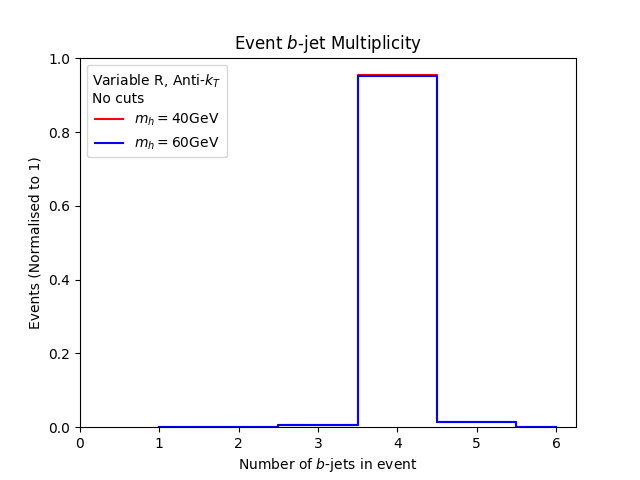
\includegraphics[scale=0.5]{plots/nbjets_varR_nocuts.png}
	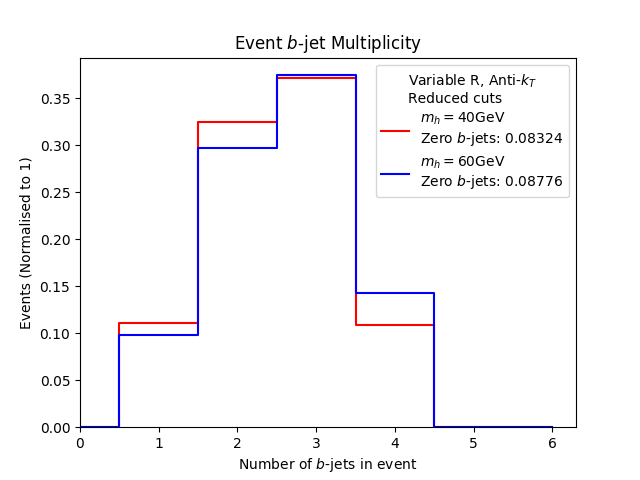
\includegraphics[scale=0.5]{plots/nbjets_varR_lowptcut.png}
	\caption{The distributions of $b$-jet multiplicities using the {variable-$R$} jet clustering algorithm. Left(Right) panel is with
no cuts(reduced $p_T$ cuts) on the $b$-jets. Note that events containing zero $b$-jets are not plotted but included in the legend, showing that,
 in the case of no cuts being applied, all events contain at least one $b$-jet.}
\label{fig:nbjets_varR}
\end{figure}


From using the variable-$R$ approach, one can extract which cone sizes have been selected in the clustering procedure.
Interestingly, one notices from Fig.~\ref{fig:Reff} that the different $h$ masses are clustered into
$b$-jets of different cone sizes. Therefore, as intimated, any experimental search strategy for our signal process using a
fixed-$R$ (whether anti-$k_T$, CA or indeed others) will not be suited to cover the entire range of possible $m_h$ values.
Furthermore, it is also evident that the sample contains $b$-jets
over a relatively large range of cone sizes. In particular, one can check the $R_{\text{eff}}$ distribution of
$p_T$ ordered $b$-jets. In Fig.~\ref{fig:Reff_bjet}, we show, in particular, the distributions of $R_{\rm eff}$ for the highest
  and lowest $p_T$ $b$-jet, from which it is evident that kinematically unbalanced events (which are far more frequent over the phase space than
balanced ones) will be largely depleted, whichever the actual fixed cone size is adopted.


\begin{figure}[htb!]
	\centering
	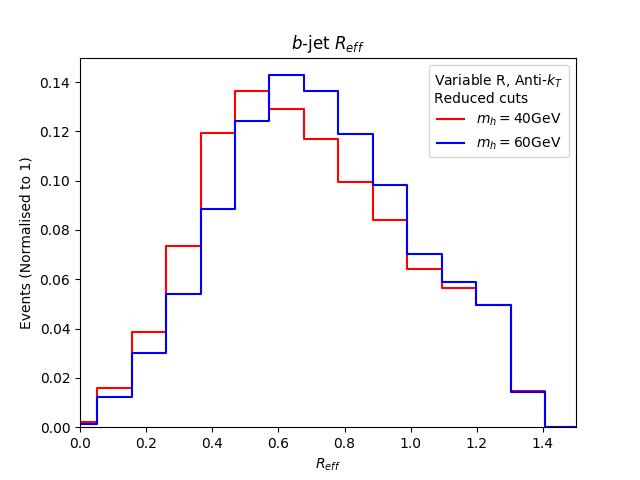
\includegraphics[scale=0.6]{plots/Reff_all.png}
	\caption{The distributions of $R_{\text{eff}}$ for all $b$-jets computed using the variable-$R$ jet clustering algorithm, upon enforcing the reduced $p_T$ cuts on the $b$-jets.}
\label{fig:Reff}
\end{figure}

\begin{figure}[htb!]
	%\centering
	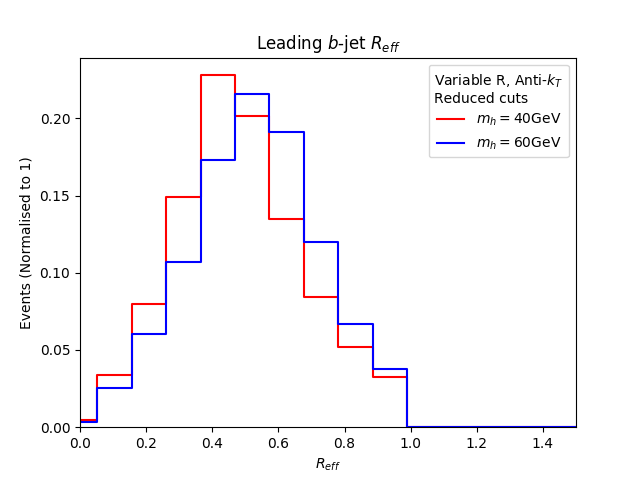
\includegraphics[scale=0.5]{plots/Reff_bjet1.png}
	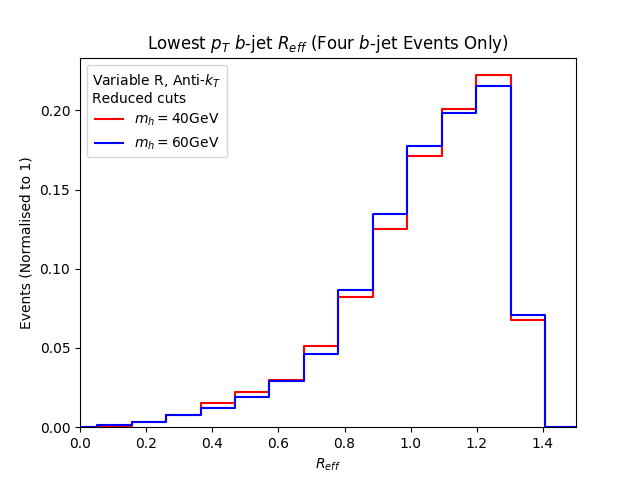
\includegraphics[scale=0.5]{plots/Reff_bjet4.png}
	\caption{The distributions of $R_{\text{eff}}$ for the highest (left) and lowest (right) $p_T$
$b$-jets computed using the variable-$R$ jet clustering algorithm, upon enforcing the reduced $p_T$ cuts on the $b$-jets.}
\label{fig:Reff_bjet}
\end{figure}

The key issue addressed by the variable-$R$ approach  thus becomes apparent. In any given event there is a
large spread in the cone sizes of the $b$-jets coming from our signal process. Using a
single fixed-$R$ value will either poorly reconstruct $m_h$ in di-jet invariant masses as it is too
low to capture the entire jet or is too large to distinguish and tag all four $b$-jets, so that this will also adversely impact the $m_H$ reconstruction. Conversely, using the variable-$R$ approach, it is possible to
extract the $m_H$ and $m_h$ resonance peaks  more efficiently. We construct all
possible di-jet invariant masses for events with at least two $b$-tagged jets and select
the one closest to the true light Higgs mass. From the left plot of Fig.~\ref{fig:invmass_ptcut_varR},
one can observe a very neatly reconstructed peak at the light Higgs boson mass. Furthermore, the four $b$-jet invariant mass
is also efficiently reproduced  around the true heavy Higgs boson mass, right plot of Fig.~\ref{fig:invmass_ptcut_varR}. Now, contrast these mass spectra with those in Fig.~\ref{fig:invmass2},  in relation to  both peak sharpness and location,
to conclude that we have been able to significantly improve the potential of extracting our signal and characterise it in terms of the underlying kinematic features. We now ought to implement the same procedure in the case of the relevant backgrounds, which we will do next.


%\begin{figure}[htb!]
%	\centering
%	\includegraphics[scale=0.5]{plots/bbbbmass_lowptcut_varR.png}
%	\includegraphics[scale=0.5]{plots/bbbbmass_nocuts.png}
%	\caption{Dijet and and four $b$-jet mass distributions, showing presence of both $m_H = 125$ GeV and $m_h = 40, 60$ GeV.}
%\label{fig:invmass_ptcut_varR}
%\end{figure}

\begin{figure}[t!]
%\centering
	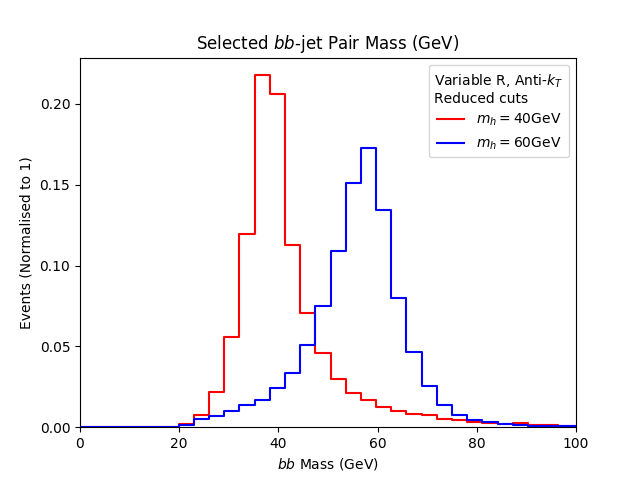
\includegraphics[scale=0.5]{plots/bbmass_varR_lowptcut.png}
%	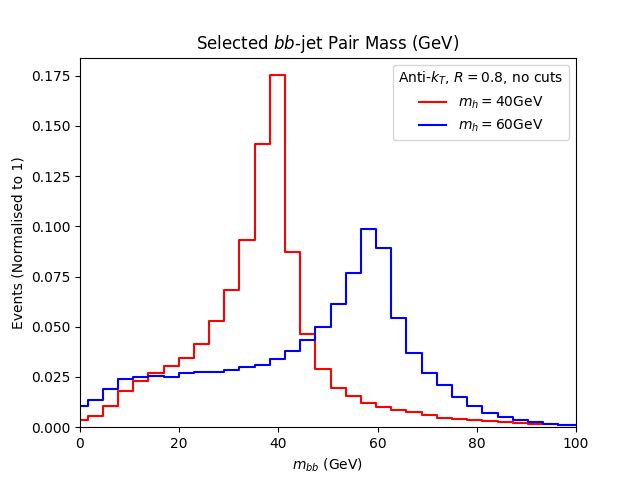
\includegraphics[scale=0.5]{plots/bbmass_AK8_nocuts.png}
	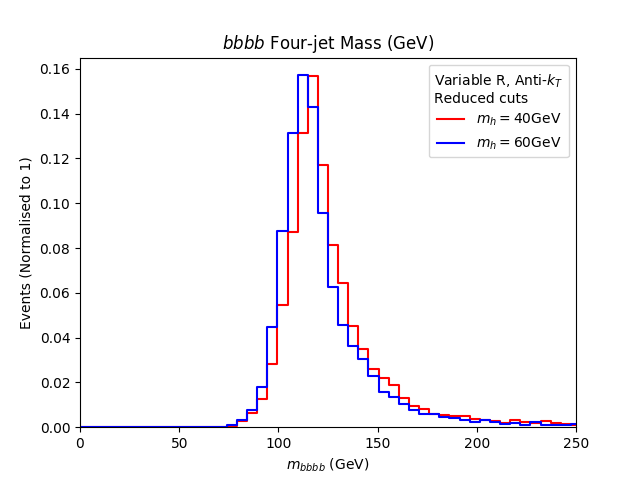
\includegraphics[scale=0.5]{plots/bbbbmass_varR_lowptcut.png}
%	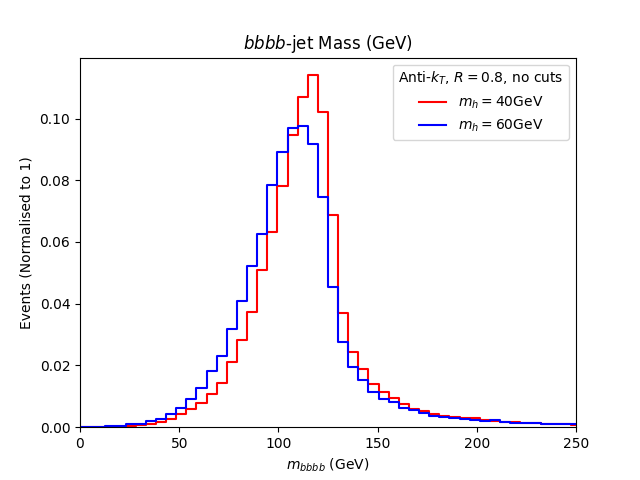
\includegraphics[scale=0.5]{plots/bbbbmass_AK8_nocuts.png}
	\caption{The distributions in invariant mass of two (left) and four (right) $b$-tagged jets, in presence of the
  reduced $p_T$ cuts on the $b$-jets. Here, we have used the variable-$R$ jet clustering algorithm.}
\label{fig:invmass_ptcut_varR}
\end{figure}

\subsection{Signal-to-Background Analysis}
As a final exercise, we perform a calculation of the signal-to-background rates, so as to compare the various jet reconstruction procedures mentioned in this paper also in connection with their performance in dealing with events not coming from our BSM process. In order to do so, we perform the selection
procedure described in Fig.~\ref{fig:selection}, which bolts on the discussed reduced $p_T$ cuts. We use the anti-$k_T$ measure throughout but conclusions would not change in case of the CA one.

\begin{figure}[!h]
\centering
\hspace*{-1.05truecm}
\begin{tikzpicture}[node distance=1.5cm]
\node (cut1) [node] {Select events that contain exactly four $b$-jets};
\node (cut2) [node, below of=cut1] {Remove event if $|m_{bbbb} - m_H|>$ 20 GeV};
\node (cut3) [node, below of=cut2] {Using di-jet pairings chosen in above analysis};
\node (cut4) [node, below of=cut3] {Remove event if $|m_{bb} - m_h|>$ 15 GeV};

\draw [arrow] (cut1) -- (cut2);
\draw [arrow] (cut2) -- (cut3);
\draw [arrow] (cut3) -- (cut4);
\end{tikzpicture}
\caption{Event selection used to compute the signal-to-background rates.}
\label{fig:selection}
\end{figure}

Tab.~\ref{tab:signalbackground1} contains the cross sections in pb for signal and the various background processes upon applying the aforementioned cuts and mass selections. It is clear from the data obtained that the QCD-induced $pp \rightarrow b\bar{b}b\bar{b}$ process  is the dominant background channel\footnote{In fact, we have computed the full four-jet sample produced by QCD, i.e., including all four-body partonic final states, yet, in presence of the described kinematical selections and $b$-tagging performances, the number of non-$b\bar bb\bar b$ events surviving is negligible.}, followed by
$pp\to Zb\bar b$ and $pp\to t\bar t$. Our next step is then to calculate the event rates in order to get the significances for two values of (integrated)  luminosity, e.g.,  ${\mathcal{L}}=$  140 and 300 fb$^{-1}$, corresponding to full Run 2 and 3 data samples, respectively. The event rate ($N$) for the various processes is given by:
%
\begin{equation}
N \ = \sigma \times \mathcal{L}.
\end{equation}
%
Tabs.~\ref{tab:signalbackground2}--\ref{tab:signalbackground3} contain $N$ values for the given two luminosities, 140 and 300 fb$^{-1}$,  respectively. After the event rates have been calculated, we simply evaluate the significance, $\Sigma$, which is given by (as a function of signal $S$ and respective background $B$ rates)
%
\begin{equation}
\Sigma = \frac{N(S)}{\sqrt{N(B_{b\bar{b}b\bar{b}})+N(B_{Zb\bar{b}})+N(B_{t\bar{t}})}}.
\end{equation}
%
It is then clear from Tabs.~\ref{tab:signalbackground4}--\ref{tab:signalbackground5}
that the variable-$R$ approach works better than the fixed-$R$ one also in providing the best significances, no matter the choices of $R$ for the latter.  The improvement in the final significances is indeed very significant.
This should not be surprising, given the ability of the former in outperforming the latter.  For completeness, we finally present in
Figs.~\ref{fig:inv_mass_bkvs_fixedR}--\ref{fig:inv_mass1234_bkvs_fixedR} the $m_{bb}$ and $m_{bbbb}$ spectra, as previously described, for the signals and  three most relevant
backgrounds (i.e., the aforementioned $b\bar bb\bar b$,  $Zb\bar b$ and $t\bar t$). Again, while the signal-to-background analysis has been performed for the
anti-$k_T$ algorithm, the same conclusions are reached for the CA case.

\begin{table}[!h]
\hspace*{-0.75truecm}
\centering
\scalebox{0.8}{
\begin{tabular}{|l|l|l|l|l|l|l|}
  \hline
  \multirow{2}{*}{Process} &
    \multicolumn{2}{c}{Var-R, $\rho=20$ GeV}\vline &
    \multicolumn{2}{c}{$R=0.4$ } \vline&
    \multicolumn{2}{c|}{$R=0.8$} \\ \cline{2-7}
  & $40$ GeV& $60$ GeV & $40$ GeV & $60$ GeV & $40$ GeV & $60$ GeV \\
  \hline
  $pp\to H\to hh  \rightarrow b\bar{b}b\bar{b}$ & 5.729$\times 10^{-3}$ &  1.306$\times 10^{-1}$&  8.483$\times 10^{-4}$& 1.658 $\times 10^{-2}$& 1.813$\times 10^{-3}$&4.193$\times 10^{-2}$ \\
  \hline
  $pp \rightarrow t\bar{t}$ & 1.226$\times 10^{-2}$ &1.635$\times 10^{-2}$ & 4.088$\times 10^{-3}$ & 1.022 $\times 10^{-2}$& 2.044$\times 10^{-3}$ & 2.044$\times 10^{-3}$ \\
  \hline
  $pp \rightarrow b\bar{b}b\bar{b}$ &3.559$\times 10^1$ &5.335$\times 10^1$&2.667$\times 10^1$& 8.891  & 1.779$\times 10^1$&2.491$\times 10^1$  \\
  \hline
  $pp \rightarrow Z b\bar{b}$ &1.797 $\times 10^{-1}$&2.471 $\times 10^{-1}$ &2.246$\times 10^{-2}$ & 4.643$\times 10^{-2}$& 7.489 $\times 10^{-2}$& 7.339  $\times 10^{-2}$ \\
  \hline
\end{tabular}
}
  \caption{\label{tab:signalbackground1} Cross sections ($pb$) of signal and background processes upon enforcing the reduced cuts plus the mass selection criteria $|m_{bbbb}-m_H|< 20$ GeV and $|m_{bb} - m_h|< 15$ GeV for the various jet reconstruction procedures.}
\end{table}

\begin{table}[ !h]
\hspace*{0.75truecm}
\scalebox{0.8}{
\begin{tabular}{|l|l|l|l|l|l|l|}
    \hline
    \multirow{2}{*}{Process} &
      \multicolumn{2}{c}{Var-R, $\rho=20$ GeV}\vline &
      \multicolumn{2}{c}{$R=0.4$ } \vline&
      \multicolumn{2}{c|}{$R=0.8$ } \\ \cline{2-7}
    & $40$ GeV& $60$ GeV & $40$ GeV & $60$ GeV & $40$ GeV & $60$ GeV \\
    \hline
    $pp\to H\to hh  \rightarrow b\bar{b}b\bar{b}$ & 802.186 & 18295.55 & 118.762 & 2322.054 &  253.862& 5870.676 \\
    \hline
    $pp \rightarrow t\bar{t}$ & 1717.052 & 2289.403 & 572.350 & 1430.877 & 286.175 & 286.175 \\
    \hline
    $pp \rightarrow b\bar{b}b\bar{b}$ &4983804&7469163.8  &3734581.2 & 1244860.54&2491902 & 3488662.8  \\
    \hline
    $pp \rightarrow Z b\bar{b}$ &25164.272&34600.874  & 3145.534 & 6500.769& 10485.112& 10275.409  \\
    \hline
  \end{tabular}
}
\caption{\label{tab:signalbackground2} Event rates of signal and backgrounds for ${\cal L}=$ $140$ fb$^{-1}$  upon enforcing the reduced cuts plus the mass selection criteria $|m_{bbbb}-m_H|< 20$ GeV and $|m_{bb} - m_h|< 15$ GeV for the various jet reconstruction procedures.}
\end{table}

\begin{table}[!h]
\hspace*{0.75truecm}
\scalebox{0.8}{
\begin{tabular}{|l|l|l|l|l|l|l|}
  \hline
  \multirow{2}{*}{Process} &
    \multicolumn{2}{c}{Var-R, $\rho=20$ GeV}\vline &
    \multicolumn{2}{c}{$R=0.4$} \vline&
    \multicolumn{2}{c|}{$R=0.8$} \\ \cline{2-7}
  & $40$ GeV& $60$ GeV & $40$ GeV & $60$ GeV & $40$ GeV & $60$ GeV \\
  \hline
  $pp\to H\to hh  \rightarrow b\bar{b}b\bar{b}$ & 1718.97 &39204.75 & 254.49 & 4975.83 &543.99& 12580.02\\
  \hline
  $pp \rightarrow t\bar{t}$ & 3679.398 & 4905.864 & 1226.466 &3066.165 & 613.233 & 613.233 \\
  \hline
  $pp \rightarrow b\bar{b}b\bar{b}$ & 10679580&16005351 &8002674&2667558.3&5339790&7475706 \\
  \hline
  $pp \rightarrow Z b\bar{b}$ &53923.44&74144.73  &6740.43 & 13930.221& 22468.098 & 22018.734  \\
  \hline
\end{tabular}
}
  \caption{\label{tab:signalbackground3} Event rates of signal and backgrounds for ${\cal L}=$ $300$ fb$^{-1}$  upon enforcing the reduced cuts plus the mass selection criteria $|m_{bbbb}-m_H|< 20$ GeV and $|m_{bb} - m_h|< 15$ GeV for the various jet reconstruction procedures.}
\end{table}

\begin{table}[!h]
\begin{center}
\scalebox{0.8}{
\begin{tabular}{ |c|c|c|c| }
 \hline
 & Var-R, $\rho=20$ GeV  & $R=0.4$ & $R=0.8$    \\
 \hline
$40~\text{GeV}$ &0.358 & 0.061 & 0.160 \\
 \hline
$60~\text{GeV}$ & 6.677&2.074 & 3.138  \\
\hline
\end{tabular}
}
\caption{\label{tab:signalbackground4} Final $\Sigma$ values calculated for signal and backgrounds for ${\cal L}=140$ fb$^{-1}$  upon enforcing the reduced cuts plus the mass selection criteria $|m_{bbbb}-m_H|< 20$ GeV and $|m_{bb} - m_h|< 15$ GeV for the various jet reconstruction procedures.}
\end{center}
\end{table}

\begin{table}[!h]
\begin{center}
\scalebox{0.8}{
\begin{tabular}{ |c|c|c|c| }
 \hline
 & Var-R, $\rho=20$ GeV  & $R=0.4$ & $R=0.8$    \\
 \hline
$40~\text{GeV}$ & 0.524 & 0.089 & 0.234 \\
 \hline
$60~\text{GeV}$  & 9.775 &3.036  & 4.594  \\
\hline
\end{tabular}
}
\caption{\label{tab:signalbackground5} Final $\Sigma$ values calculated for signal and backgrounds for ${\cal L}=300$ fb$^{-1}$  upon enforcing the reduced cuts plus the mass selection criteria $|m_{bbbb}-m_H|< 20$ GeV and $|m_{bb} - m_h|< 15$ GeV for the various jet reconstruction procedures.}
\end{center}
\end{table}

\subsection{Discussion}
Before discussing our results in detail and concluding, we address some points here, as well as reviewing some other studies utilising a variable-$R$ reconstruction procedure.

In Fig.~\ref{fig:Reff_bjet} we note that, while the leading $b$-jet has an $R_{\text{eff}}$ roughly in line with expected values ($R_{\text{eff}} \simeq 0.5$), the lowest $p_T$ $b$-jets have large cone sizes ($R_{\text{eff}} > 1.0$), risking potential contamination from additional radiation. This effect is discussed in \cite{Lapsien:2016zor}. We do not implement any such vetoes to remedy this effect, however despite this our results still suggest variable-$R$ displays an improvement over traditional methods. 

There have been other studies utilising variable-$R$ methods for physics searches. For example, in highly boosted object tagging of $hh \rightarrow bb\bar{b}\bar{b}$ decays in \cite{ATLAS:2016hcf}. Futhermore, in \cite{Lapsien:2016zor} mentioned above, a variable-$R$ algorithm is deployed in the context of heavy particle decays. In both examples, an improvement over current fixed R methods are present when using variable-$R$, which is in line with our findings.

As a final word on using variable-$R$ jet reconstruction in experiments. In particular, the studies \cite{ATLAS:2017juw, ATLAS:2020udg} explore the possibility of Higgs to $b$-jet tagging at ATLAS using variable-$R$ techniques. Specifically these studies deal with boosted topologies, focusing on fat $b$-jet substructure, so the validity of applying these techniques in a non boosted regime is to be determined. 

\section{Conclusions}
In this paper, we have assessed the potential scope of the LHC
experiments in accessing BSM Higgs signals induced by cascade decays
of the 125 GeV SM-like Higgs state discovered in July 2012, through
the following prototypical production and decay channel: $gg\to H\to
hh$, where $H$ is the SM-like Higgs state and $h$ is a lighter BSM
Higgs state, with mass less than $m_H/2$, so as to induce resonant
production and decay, thereby enhancing the overall rate. Any such a
$h$ boson, largely independently of the BSM construct hosting it,
would decay to $b\bar b$ pairs, eventually leading to a four $b$
signature. The latter is extremely difficult to establish at the LHC,
owing to the substantial hadronic background. Therefore,
$b$-tagging techniques are to be exploited in order to make such a
signal visible. However, this poses the problem that the latter are
most efficient at large transverse momentum of the $b$-jets, say at
least 20 GeV, which in turn corresponds to a significant loss of
signal events if the BSM Higgs mass is in the sub-60 GeV range. Hence,
if one intends to maximise sensitivity to this benchmark signature of
BSM physics, a thorough reassessment of the current Run 2 approaches
is mandated for, and especially so in view of the upcoming Run 3. 

The first message we deliver is that, with current $p_T$ limitations on final state $b$-jets, using a fixed-$R$ jet reconstruction and tagging procedure will lead to a poor signal visibility, with a majority of signal $b$-jets being lost. We present a reduced cut flow, based on existing $b\bar b\mu^+\mu^-$ analyses, and show that this indeed provides a window into final states of $gg \rightarrow H \rightarrow hh \rightarrow bb\bar{b}\bar{b}$ decays with $m_H = 125$ GeV and $m_h < \frac{m_H}{2}$. 

Additionally, and perhaps more remarkably, we also test a variable-$R$ reconstruction approach on events with this reduced cut flow, and show a significant improvement in signal yield, as well as signal-to-background rates. We notice that in final states of this kind, the signal $b$-jets have a wide range of $p_T$, and hence varied spread of constituents. Using a fixed cone of a standard size ($R=0.4$) well constructs higher $p_T$ jets in an event, but does not capture much of the wider angle radiation from lower $p_T$ jets. This leads to two issues: firstly it will prove difficult to accurately construct $m_h$ and $M_H$ in the dijet and four-jet invariant masses. Secondly, these jets will more often be lost due to kinematic cuts. A larger cone ($R=0.8$) on the other hand, will gather up too much `junk' in the higher $p_T$ jets, which again will contaminate the signal.

As we have obtained all of the above in presence of sophisticated MC event simulation, based on exact  scattering MEs, state-of-the-art parton shower, hadronisation and $B$-hadron decays as well as a realistic detector simulation, we recommend deployment of our envisaged selection strategy in future LHC analyses aiming at extracting the aforementioned decay chain. In fact, while we have quantitatively based our case on the example of the 2HDM-II (wherein $h$ was the lightest CP-even Higgs state, yet it could equally have been the CP-odd one, $A$), our procedure can identically be used in other BSM constructs featurings light (pseudo)scalar states emerging from decays of the SM-like Higgs state and in turn decaying into $b\bar b$ pairs.


\section*{Acknowledgments}
SM is supported also in part through the NExT Institute and the STFC Consolidated Grant No. ST/L000296/1. BF is funded by the DISCnet SEPnet scholarship scheme. The work of AC is funded by the Department of Science and Technology, Government of India, under Grant No. IFA18-PH 224 (INSPIRE Faculty Award).

We all thank G.P. Salam for useful advice. We give thanks to Benjamin Fuks, Eric Conte and others in the MadAnalysis5 team for their assistance with technical queries.

BF and SJ acknowledge the use of the IRIDIS High Performance Computing Facility, and associated support services at the University of Southampton, in the completion of this work.

{\textcolor{red}{SM: others?}}

%%------------------------------------------------------------------------------------
%%% -- References
%%------------------------------------------------------------------------------------
%\clearpage

\begin{thebibliography}{99}

%\cite{Aad:2012tfa}
\bibitem{Aad:2012tfa}
  G.~Aad {\it et al.} [ATLAS Collaboration],
  %``Observation of a new particle in the search for the Standard Model Higgs boson with the ATLAS detector at the LHC,''
  Phys.\ Lett.\ B {\bf 716} (2012) 1
  doi:10.1016/j.physletb.2012.08.020
  [arXiv:1207.7214 [hep-ex]].
  %%CITATION = doi:10.1016/j.physletb.2012.08.020;%%
  %11193 citations counted in INSPIRE as of 04 Aug 2020

%\cite{Book}
\bibitem{Book}
  K.~Shaaban and S.~Moretti,,
  ``Supersymmetry Beyond Minimality: from Theory to Experiment'',
  CRC Press (Taylor \& Francis), 2017.

%\cite{Ellwanger:2009dp}
\bibitem{Ellwanger:2009dp}
  U.~Ellwanger, C.~Hugonie and A.~M.~Teixeira,
  %``The Next-to-Minimal Supersymmetric Standard Model,''
  Phys.\ Rept.\  {\bf 496} (2010) 1
  doi:10.1016/j.physrep.2010.07.001
  [arXiv:0910.1785 [hep-ph]].
  %%CITATION = doi:10.1016/j.physrep.2010.07.001;%%
  %980 citations counted in INSPIRE as of 04 Aug 2020


%\cite{Gunion:1989we}
\bibitem{Gunion:1989we}
  J.~F.~Gunion, H.~E.~Haber, G.~L.~Kane and S.~Dawson,
  %``The Higgs Hunter's Guide,''
  Front.\ Phys.\  {\bf 80} (2000) 1.
  %%CITATION = FRPHA,80,1;%%
  %1125 citations counted in INSPIRE as of 04 Aug 2020


%\cite{Gunion:1992hs}
\bibitem{Gunion:1992hs}
  J.~F.~Gunion, H.~E.~Haber, G.~L.~Kane and S.~Dawson,
  %``Errata for the Higgs hunter's guide,''
  hep-ph/9302272.
  %%CITATION = HEP-PH/9302272;%%
  %165 citations counted in INSPIRE as of 04 Aug 2020


%\cite{Branco:2011iw}
\bibitem{Branco:2011iw}
  G.~C.~Branco, P.~M.~Ferreira, L.~Lavoura, M.~N.~Rebelo, M.~Sher and J.~P.~Silva,
  %``Theory and phenomenology of two-Higgs-doublet models,''
  Phys.\ Rept.\  {\bf 516} (2012) 1
  doi:10.1016/j.physrep.2012.02.002
  [arXiv:1106.0034 [hep-ph]].
  %%CITATION = doi:10.1016/j.physrep.2012.02.002;%%
  %1797 citations counted in INSPIRE as of 04 Aug 2020


%\cite{Moretti:1994ds}
\bibitem{Moretti:1994ds}
  S.~Moretti and W.~J.~Stirling,
  %``Contributions of below threshold decays to MSSM Higgs branching ratios,''
  Phys.\ Lett.\ B {\bf 347} (1995) 291
   Erratum: [Phys.\ Lett.\ B {\bf 366} (1996) 451]
  doi:10.1016/0370-2693(95)00088-3, 10.1016/0370-2693(95)01477-2
  [hep-ph/9412209, hep-ph/9511351].
  %%CITATION = doi:10.1016/0370-2693(95)00088-3, 10.1016/0370-2693(95)01477-2;%%
  %97 citations counted in INSPIRE as of 04 Aug 2020


%\cite{Djouadi:1995gv}
\bibitem{Djouadi:1995gv}
  A.~Djouadi, J.~Kalinowski and P.~M.~Zerwas,
  %``Two and three-body decay modes of SUSY Higgs particles,''
  Z.\ Phys.\ C {\bf 70} (1996) 435
  doi:10.1007/s002880050121
  [hep-ph/9511342].
  %%CITATION = doi:10.1007/s002880050121;%%
  %202 citations counted in INSPIRE as of 04 Aug 2020


%\cite{Scodellaro:2017wli}
\bibitem{Scodellaro:2017wli}
  L.~Scodellaro [ATLAS and CMS Collaborations],
  %``b tagging in ATLAS and CMS,''
  arXiv:1709.01290 [hep-ex].
  %%CITATION = ARXIV:1709.01290;%%
  %5 citations counted in INSPIRE as of 04 Aug 2020


%\cite{Krohn:2009zg}
\bibitem{Krohn:2009zg}
  D.~Krohn, J.~Thaler and L.~T.~Wang,
  %``Jets with Variable R,''
  JHEP {\bf 0906} (2009) 059
  doi:10.1088/1126-6708/2009/06/059
  [arXiv:0903.0392 [hep-ph]].
  %%CITATION = doi:10.1088/1126-6708/2009/06/059;%%
  %92 citations counted in INSPIRE as of 04 Aug 2020


%\cite{Sterman:1977wj}
\bibitem{Sterman:1977wj}
  G.~F.~Sterman and S.~Weinberg,
  %``Jets from Quantum Chromodynamics,''
  Phys.\ Rev.\ Lett.\  {\bf 39} (1977) 1436.
  doi:10.1103/PhysRevLett.39.1436
  %%CITATION = doi:10.1103/PhysRevLett.39.1436;%%
  %1024 citations counted in INSPIRE as of 04 Aug 2020


%\cite{Moretti:1998qx}
\bibitem{Moretti:1998qx}
  S.~Moretti, L.~Lonnblad and T.~Sjostrand,
  %``New and old jet clustering algorithms for electron - positron events,''
  JHEP {\bf 9808} (1998) 001
  doi:10.1088/1126-6708/1998/08/001
  [hep-ph/9804296].
  %%CITATION = doi:10.1088/1126-6708/1998/08/001;%%
  %103 citations counted in INSPIRE as of 04 Aug 2020


%\cite{Cacciari:2011ma}
\bibitem{Cacciari:2011ma}
  M.~Cacciari, G.~P.~Salam and G.~Soyez,
  %``FastJet User Manual,''
  Eur.\ Phys.\ J.\ C {\bf 72} (2012) 1896
  doi:10.1140/epjc/s10052-012-1896-2
  [arXiv:1111.6097 [hep-ph]].
  %%CITATION = doi:10.1140/epjc/s10052-012-1896-2;%%
  %3629 citations counted in INSPIRE as of 04 Aug 2020


%\cite{Wobisch:1998wt}
\bibitem{Wobisch:1998wt}
  M.~Wobisch and T.~Wengler,
  %``Hadronization corrections to jet cross-sections in deep inelastic scattering,''
  In *Hamburg 1998/1999, Monte Carlo generators for HERA physics* 270-279
  [hep-ph/9907280].
  %%CITATION = HEP-PH/9907280;%%
  %602 citations counted in INSPIRE as of 04 Aug 2020


%\cite{Dokshitzer:1997in}
\bibitem{Dokshitzer:1997in}
  Y.~L.~Dokshitzer, G.~D.~Leder, S.~Moretti and B.~R.~Webber,
  %``Better jet clustering algorithms,''
  JHEP {\bf 9708} (1997) 001
  doi:10.1088/1126-6708/1997/08/001
  [hep-ph/9707323].
  %%CITATION = doi:10.1088/1126-6708/1997/08/001;%%
  %1158 citations counted in INSPIRE as of 04 Aug 2020


%\cite{Cacciari:2008gp}
\bibitem{Cacciari:2008gp}
  M.~Cacciari, G.~P.~Salam and G.~Soyez,
  %``The anti-$k_t$ jet clustering algorithm,''
  JHEP {\bf 0804} (2008) 063
  doi:10.1088/1126-6708/2008/04/063
  [arXiv:0802.1189 [hep-ph]].
  %%CITATION = doi:10.1088/1126-6708/2008/04/063;%%
  %7207 citations counted in INSPIRE as of 04 Aug 2020


%\cite{Salam:2009jx}
\bibitem{Salam:2009jx}
  G.~P.~Salam,
  %``Towards Jetography,''
  Eur.\ Phys.\ J.\ C {\bf 67} (2010) 637
  doi:10.1140/epjc/s10052-010-1314-6
  [arXiv:0906.1833 [hep-ph]].
  %%CITATION = doi:10.1140/epjc/s10052-010-1314-6;%%
  %560 citations counted in INSPIRE as of 04 Aug 2020


%\cite{Sirunyan:2017ezt}
\bibitem{Sirunyan:2017ezt}
  A.~M.~Sirunyan {\it et al.} [CMS Collaboration],
  %``Identification of heavy-flavour jets with the CMS detector in pp collisions at 13 TeV,''
  JINST {\bf 13} (2018) no.05,  P05011
  doi:10.1088/1748-0221/13/05/P05011
  [arXiv:1712.07158 [physics.ins-det]].
  %%CITATION = doi:10.1088/1748-0221/13/05/P05011;%%
  %455 citations counted in INSPIRE as of 04 Aug 2020

\bibitem{DEEPJET}
A.~M.~Sirunyan {\it et al.} [CMS Collaboration],
%"Performance of the DeepJet b tag- ging algorithm using 41.9/fb of data from proton-proton collisions at 13TeV with Phase 1 CMS detector" 
Tech. Rep. CMS-DP-2018-058 (2018).


%\cite{Sirunyan:2018mot}
\bibitem{Sirunyan:2018mot}
  A.~M.~Sirunyan {\it et al.} [CMS Collaboration],
  %``Search for an exotic decay of the Higgs boson to a pair of light pseudoscalars in the final state with two muons and two b quarks in pp collisions at 13 TeV,''
  Phys.\ Lett.\ B {\bf 795} (2019) 398
  doi:10.1016/j.physletb.2019.06.021
  [arXiv:1812.06359 [hep-ex]].
  %%CITATION = doi:10.1016/j.physletb.2019.06.021;%%
  %18 citations counted in INSPIRE as of 04 Aug 2020


%\cite{Eriksson:2010zzb}
\bibitem{Eriksson:2010zzb}
  D.~Eriksson, J.~Rathsman and O.~Stal,
  %``2HDMC: Two-Higgs-doublet model calculator,''
  Comput.\ Phys.\ Commun.\  {\bf 181} (2010) 833.
  doi:10.1016/j.cpc.2009.12.016
  %%CITATION = doi:10.1016/j.cpc.2009.12.016;%%
  %59 citations counted in INSPIRE as of 04 Aug 2020


%\cite{Bechtle:2013wla}
\bibitem{Bechtle:2013wla}
  P.~Bechtle, O.~Brein, S.~Heinemeyer, O.~Stål, T.~Stefaniak, G.~Weiglein and K.~E.~Williams,
  %``$\mathsf{HiggsBounds}-4$: Improved Tests of Extended Higgs Sectors against Exclusion Bounds from LEP, the Tevatron and the LHC,''
  Eur.\ Phys.\ J.\ C {\bf 74} (2014) no.3,  2693
  doi:10.1140/epjc/s10052-013-2693-2
  [arXiv:1311.0055 [hep-ph]].
  %%CITATION = doi:10.1140/epjc/s10052-013-2693-2;%%
  %417 citations counted in INSPIRE as of 04 Aug 2020


%\cite{Bechtle:2013xfa}
\bibitem{Bechtle:2013xfa}
  P.~Bechtle, S.~Heinemeyer, O.~Stål, T.~Stefaniak and G.~Weiglein,
  %``$HiggsSignals$: Confronting arbitrary Higgs sectors with measurements at the Tevatron and the LHC,''
  Eur.\ Phys.\ J.\ C {\bf 74} (2014) no.2,  2711
  doi:10.1140/epjc/s10052-013-2711-4
  [arXiv:1305.1933 [hep-ph]].
  %%CITATION = doi:10.1140/epjc/s10052-013-2711-4;%%
  %391 citations counted in INSPIRE as of 04 Aug 2020


%\cite{Mahmoudi:2009zz}
\bibitem{Mahmoudi:2009zz}
  F.~Mahmoudi,
  %``SuperIso v3.0, flavor physics observables calculations: Extension to NMSSM,''
  Comput.\ Phys.\ Commun.\  {\bf 180} (2009) 1718.
  doi:10.1016/j.cpc.2009.05.001
  %%CITATION = doi:10.1016/j.cpc.2009.05.001;%%
  %70 citations counted in INSPIRE as of 04 Aug 2020


%\cite{Ball:2014uwa}
\bibitem{Ball:2014uwa}
  R.~D.~Ball {\it et al.} [NNPDF Collaboration],
  %``Parton distributions for the LHC Run II,''
  JHEP {\bf 1504} (2015) 040
  doi:10.1007/JHEP04(2015)040
  [arXiv:1410.8849 [hep-ph]].
  %%CITATION = doi:10.1007/JHEP04(2015)040;%%
  %2209 citations counted in INSPIRE as of 04 Aug 2020


%\cite{Alwall:2014hca}
\bibitem{Alwall:2014hca}
  J.~Alwall {\it et al.},
  %``The automated computation of tree-level and next-to-leading order differential cross sections, and their matching to parton shower simulations,''
  JHEP {\bf 1407} (2014) 079
  doi:10.1007/JHEP07(2014)079
  [arXiv:1405.0301 [hep-ph]].
  %%CITATION = doi:10.1007/JHEP07(2014)079;%%
  %4855 citations counted in INSPIRE as of 04 Aug 2020


%\cite{Sjostrand:2007gs}
\bibitem{Sjostrand:2007gs}
  T.~Sjostrand, S.~Mrenna and P.~Z.~Skands,
  %``A Brief Introduction to PYTHIA 8.1,''
  Comput.\ Phys.\ Commun.\  {\bf 178} (2008) 852
  doi:10.1016/j.cpc.2008.01.036
  [arXiv:0710.3820 [hep-ph]].
  %%CITATION = doi:10.1016/j.cpc.2008.01.036;%%
  %5401 citations counted in INSPIRE as of 04 Aug 2020


%\cite{Conte:2012fm}
\bibitem{Conte:2012fm}
  E.~Conte, B.~Fuks and G.~Serret,
  %``MadAnalysis 5, A User-Friendly Framework for Collider Phenomenology,''
  Comput.\ Phys.\ Commun.\  {\bf 184} (2013) 222
  doi:10.1016/j.cpc.2012.09.009
  [arXiv:1206.1599 [hep-ph]].
  %%CITATION = doi:10.1016/j.cpc.2012.09.009;%%
  %341 citations counted in INSPIRE as of 04 Aug 2020


%\cite{Conte:2018vmg}
\bibitem{Conte:2018vmg}
  E.~Conte and B.~Fuks,
  %``Confronting new physics theories to LHC data with MADANALYSIS 5,''
  Int.\ J.\ Mod.\ Phys.\ A {\bf 33} (2018) no.28,  1830027
  doi:10.1142/S0217751X18300272
  [arXiv:1808.00480 [hep-ph]].
  %%CITATION = doi:10.1142/S0217751X18300272;%%
  %28 citations counted in INSPIRE as of 04 Aug 2020


%\cite{Sirunyan:2019jud}
\bibitem{Sirunyan:2019jud}
  A.~M.~Sirunyan {\it et al.} [CMS Collaboration],
  %``Measurement of the $\mathrm{t\bar{t}}\mathrm{b\bar{b}}$ production cross section in the all-jet final state in pp collisions at $\sqrt{s} =$ 13 TeV,''
  Phys.\ Lett.\ B {\bf 803} (2020) 135285
  doi:10.1016/j.physletb.2020.135285
  [arXiv:1909.05306 [hep-ex]].
  %%CITATION = doi:10.1016/j.physletb.2020.135285;%%
  %5 citations counted in INSPIRE as of 04 Aug 2020


%\cite{Lapsien:2016zor}
\bibitem{Lapsien:2016zor}
  T.~Lapsien, R.~Kogler and J.~Haller,
  %``A new tagger for hadronically decaying heavy particles at the LHC,''
  Eur.\ Phys.\ J.\ C {\bf 76} (2016) no.11,  600
  doi:10.1140/epjc/s10052-016-4443-8
  [arXiv:1606.04961 [hep-ph]].
  %%CITATION = doi:10.1140/epjc/s10052-016-4443-8;%%
  %17 citations counted in INSPIRE as of 04 Aug 2020


%\cite{ATLAS:2016hcf}
\bibitem{ATLAS:2016hcf}
  The ATLAS collaboration [ATLAS Collaboration],
  %``Boosted Object Tagging with Variable-$R$ Jets in the ATLAS Detector,''
  ATL-PHYS-PUB-2016-013.
  %%CITATION = ATL-PHYS-PUB-2016-013;%%
  %13 citations counted in INSPIRE as of 04 Aug 2020


%\cite{ATLAS:2017juw}
\bibitem{ATLAS:2017juw}
  The ATLAS collaboration [ATLAS Collaboration],
  %``Variable Radius, Exclusive-k$_{T}$, and Center-of-Mass Subjet Reconstruction for Higgs($\rightarrow b\bar{b}$) Tagging in ATLAS,''
  ATL-PHYS-PUB-2017-010.
  %%CITATION = ATL-PHYS-PUB-2017-010;%%
  %30 citations counted in INSPIRE as of 04 Aug 2020


%\cite{ATLAS:2020udg}
\bibitem{ATLAS:2020udg}
  The ATLAS collaboration [ATLAS Collaboration],
  %``Measurement of the associated production of a Higgs boson decaying to $b$ quarks with a vector boson at high transverse momentum in $pp$ collisions at $\sqrt{s} = 13$ TeV with the ATLAS detector,''
  ATLAS-CONF-2020-007.
  %%CITATION = ATLAS-CONF-2020-007;%%
  %5 citations counted in INSPIRE as of 04 Aug 2020


\end{thebibliography}
%%%%%%%%%%%%%%%%%%%%%%%%%%%%%%%%%%%%%%%%%%%%%%%%%%%%%%%%%%%%%%%%%%%%%%%%%%%%%%%%%%%%%
%%%%%%%%%%%%%%%%%%%%%%%%%%%%%%%%%%%%%%%%%%%%%%%%%%%%%%%%%%%%%%%%%%%%%%%%%%%%%%%%%%%%%

\clearpage
\thispagestyle{empty}

\begin{figure}[t!]
\hspace*{-0.25cm}
	%\centering
    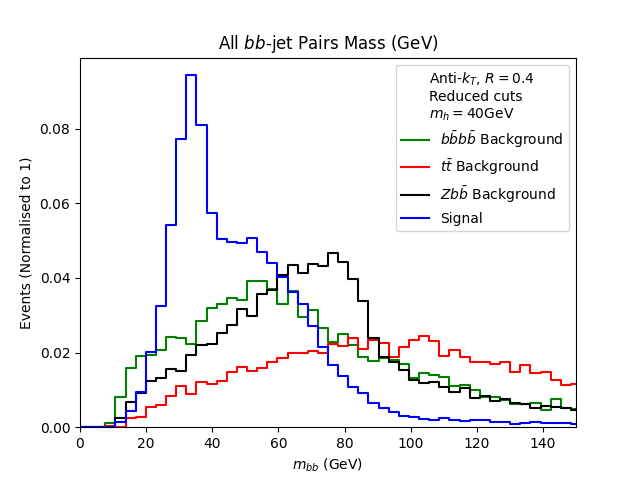
\includegraphics[scale=0.5]{plots/Background/bb_mass_all_pairs_40gev_AK4.png}
    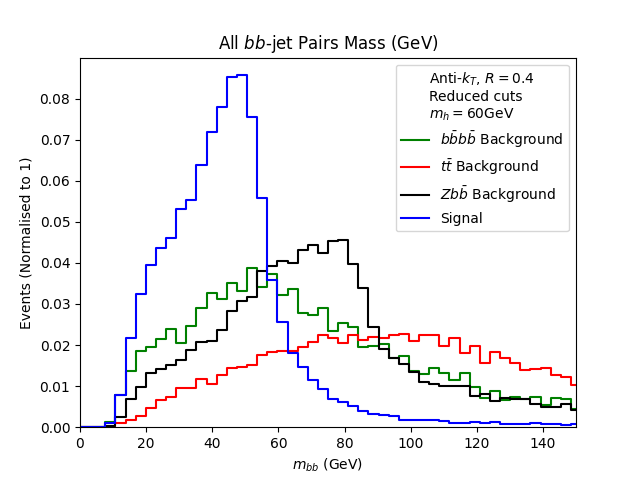
\includegraphics[scale=0.5]{plots/Background/bb_mass_all_pairs_60gev_AK4.png}
    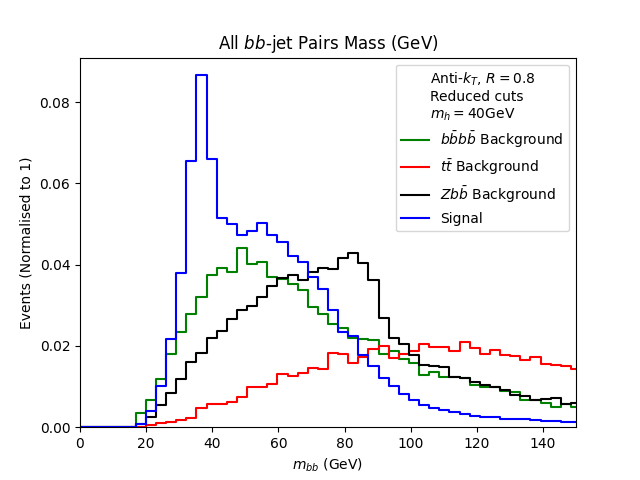
\includegraphics[scale=0.5]{plots/Background/bb_mass_all_pairs_40gev_AK8.png}
    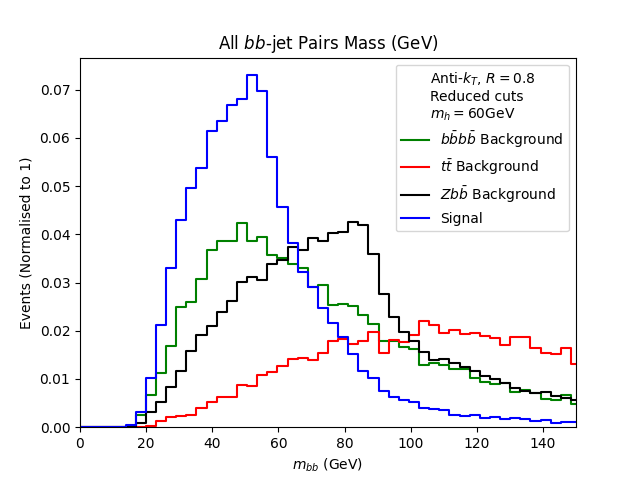
\includegraphics[scale=0.5]{plots/background/bb_mass_all_pairs_60gev_AK8.png}
    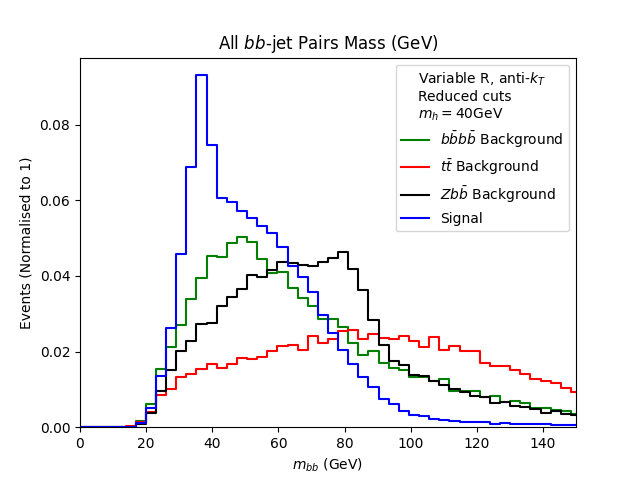
\includegraphics[scale=0.5]{plots/background/bb_mass_all_pairs_40gev_rho20.png}
    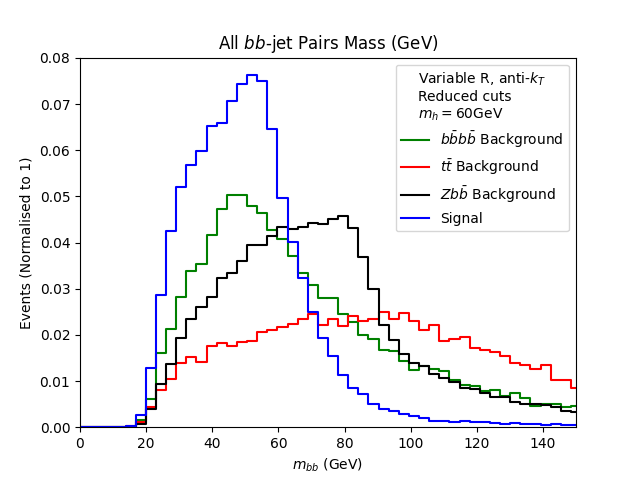
\includegraphics[scale=0.5]{plots/background/bb_mass_all_pairs_60gev_rho20.png}
	\caption{The distributions in invariant mass of two $b$-jets for signals and backgrounds after the reduced $p_T$ cuts plus the discussed mass selections
for fixed-$R$ ($R=0.4$ at the top and 0.8 in the middle) and variable-$R$ ($\rho=20$ GeV at the bottom) jet clustering.}
\label{fig:inv_mass_bkvs_fixedR}
\end{figure}

\clearpage
\thispagestyle{empty}

\begin{figure}[t!]
\hspace*{-0.25cm}
%	\centering
    \includegraphics[scale=0.5]{plots/Background/bbbb_mass_40gev_AK4.png}
    \includegraphics[scale=0.5]{plots/Background/bbbb_mass_60gev_AK4.png}
    \includegraphics[scale=0.5]{plots/Background/bbbb_mass_40gev_AK8.png}
    \includegraphics[scale=0.5]{plots/Background/bbbb_mass_60gev_AK8.png}
    \includegraphics[scale=0.5]{plots/Background/bbbb_mass_40gev_rho20.png}
    \includegraphics[scale=0.5]{plots/Background/bbbb_mass_60gev_rho20.png}
	\caption{The distributions in invariant mass of four $b$-jets for signals and backgrounds after the reduced $p_T$ cuts plus the discussed mass selections
for fixed-$R$ ($R=0.4$ at the top and 0.8 in the middle) and variable-$R$ ($\rho=20$ GeV at the bottom) jet clustering.}
\label{fig:inv_mass1234_bkvs_fixedR}
\end{figure}


\end{document}
